% SCE 513 Course Project -- M4 final report (IFAC two-column layout)
% Every result number is a macro from ../results/numbers.tex (M3 scripts) or
% ../results/numbers_m4.tex (m4_analysis.py). Do not type numbers by hand.
\documentclass[10pt,a4paper,twocolumn]{article}
\usepackage[a4paper,left=17mm,right=17mm,top=20mm,bottom=25mm,columnsep=8mm]{geometry}
\usepackage[T1]{fontenc}
\usepackage{mathptmx}\renewcommand{\ttdefault}{pcr}
\usepackage{amsmath,amssymb}
\usepackage{graphicx,booktabs,multirow,xcolor}
\usepackage[round,authoryear]{natbib}
\usepackage[font=footnotesize,labelfont=bf,labelsep=period]{caption}
\usepackage{titlesec}
\usepackage[hidelinks]{hyperref}
\usepackage{microtype}\usepackage{placeins}\usepackage{dblfloatfix}\usepackage{tikz}\usetikzlibrary{arrows.meta,positioning}
\titleformat{\section}{\normalfont\normalsize\bfseries\centering}{\thesection.}{0.5em}{\MakeUppercase}
\titleformat{\subsection}{\normalfont\normalsize\itshape}{\thesubsection}{0.5em}{}
\titlespacing*{\section}{0pt}{8pt}{4pt}
\titlespacing*{\subsection}{0pt}{5pt}{2pt}
\setlength{\parindent}{0pt}\setlength{\parskip}{3pt}
\setlength{\textfloatsep}{8pt}\setlength{\floatsep}{6pt}
\setlength{\abovecaptionskip}{3pt}
\graphicspath{{../results/}}
% generated by make_figures.py -- do not edit by hand
\newcommand{\nCinit}{252.57}
\newcommand{\nCopt}{1.217}
\newcommand{\nRatio}{207.5}
\newcommand{\nNit}{1000}
\newcommand{\nNfev}{1141}
\newcommand{\nTmin}{6.5}
\newcommand{\nCFinit}{3.20}
\newcommand{\nCFopt}{3.10}
\newcommand{\nCFschA}{1.879}
\newcommand{\nCFschB}{1.896}
\newcommand{\nCsch}{159.0}
\newcommand{\nCschB}{158.9}
\newcommand{\nKapInit}{36.9}
\newcommand{\nKapOpt}{59.3}
\newcommand{\nKapSch}{34.7}
\newcommand{\nInInit}{99.2}
\newcommand{\nInOpt}{90.1}
\newcommand{\nInSch}{93.8}
\newcommand{\ndA}{1.2e-12}
\newcommand{\nSSrelOpt}{1.4e-13}
\newcommand{\nSSpOpt}{5}
\newcommand{\nSSpInit}{5}
\newcommand{\nRelCinit}{-12.0}
\newcommand{\nRelCopt}{-68.6}
\newcommand{\nRelCFsch}{0.5}
\newcommand{\nRelCFopt}{-15.5}
\newcommand{\nGridInit}{230.4}
\newcommand{\nGridOpt}{1.103}
\newcommand{\nGridRatio}{208.8}
\newcommand{\nXzeroInit}{8.9e-15}
\newcommand{\nXzeroOpt}{2.6e-14}
\newcommand{\nPtenOpt}{5.1e-14}
\newcommand{\nDiagPass}{8}
\newcommand{\nDiagN}{8}
\newcommand{\nEpsInitA}{1829.9}
\newcommand{\nEpsOptA}{1.221}
\newcommand{\nEpsRatioA}{1498.1}
\newcommand{\nEpsInitB}{252.6}
\newcommand{\nEpsOptB}{1.217}
\newcommand{\nEpsRatioB}{207.5}
\newcommand{\nEpsInitC}{97.7}
\newcommand{\nEpsOptC}{1.208}
\newcommand{\nEpsRatioC}{80.9}
\newcommand{\nEpsInitD}{34.4}
\newcommand{\nEpsOptD}{1.179}
\newcommand{\nEpsRatioD}{29.2}
\newcommand{\nCoptAtCap}{1.439}
\newcommand{\nBinLoInit}{30}
\newcommand{\nBinLoOpt}{67}
\newcommand{\nBinHiInit}{34}
\newcommand{\nBinHiOpt}{70}
\newcommand{\nRelCbudget}{20.5}
\newcommand{\nCbudget}{4.67}
\newcommand{\nFirstBelow}{18}
\newcommand{\nP}{8}
\newcommand{\nSSrelInit}{2.4e-13}
\newcommand{\nOldCopt}{1.211}
\newcommand{\nOldSSrel}{2.5e-05}
\newcommand{\nOldSSp}{6}
\newcommand{\nEaC}{4.17}
\newcommand{\nEaR}{60.6}
\newcommand{\nEaCF}{3.31}
\newcommand{\nEaIt}{16}
\newcommand{\nEbC}{3.29}
\newcommand{\nEbR}{76.8}
\newcommand{\nEbCF}{3.34}
\newcommand{\nEbIt}{20}
\newcommand{\nEcC}{2.66}
\newcommand{\nEcR}{94.8}
\newcommand{\nEcCF}{3.16}
\newcommand{\nEcIt}{25}
\newcommand{\nAdamFinal}{1.916}
\newcommand{\nAdamSixteen}{26.9}
\newcommand{\nAdamSteps}{400}
\newcommand{\nAdamCF}{3.83}
\newcommand{\nMCiMean}{249.0}
\newcommand{\nMCiMedian}{251.5}
\newcommand{\nMCiQone}{210.9}
\newcommand{\nMCiQthree}{279.7}
\newcommand{\nMCiMin}{118.7}
\newcommand{\nMCiMax}{408.2}
\newcommand{\nMCoMean}{1.24}
\newcommand{\nMCoMedian}{1.21}
\newcommand{\nMCoQone}{1.18}
\newcommand{\nMCoQthree}{1.23}
\newcommand{\nMCoMin}{1.13}
\newcommand{\nMCoMax}{1.84}
\newcommand{\nMCbMean}{7.32}
\newcommand{\nMCbMedian}{5.62}
\newcommand{\nMCbQone}{4.41}
\newcommand{\nMCbQthree}{10.21}
\newcommand{\nMCbMin}{3.22}
\newcommand{\nMCbMax}{15.09}
\newcommand{\nMCtMean}{4.06}
\newcommand{\nMCtMedian}{3.65}
\newcommand{\nMCtQone}{3.17}
\newcommand{\nMCtQthree}{4.59}
\newcommand{\nMCtMin}{2.47}
\newcommand{\nMCtMax}{9.28}
\newcommand{\nMCn}{20}
\newcommand{\nMCratio}{203.0}
\newcommand{\nMCratioB}{40.3}
\newcommand{\nMCnit}{995}
\newcommand{\nMCtime}{6.4}
\newcommand{\nMCinRange}{10}
\newcommand{\nMCkMed}{18.5}
\newcommand{\nMCkMin}{13}
\newcommand{\nMCkMax}{32}

% generated by m4_analysis.py -- do not edit by hand
\newcommand{\mNMC}{20}
\newcommand{\mRerunIdentical}{9}
\newcommand{\mRerunFinalMax}{3.5}
\newcommand{\mRerunFinalMed}{0.4}
\newcommand{\mRerunItTwentyMax}{1e-06}
\newcommand{\mCsixteenMed}{4.45}
\newcommand{\mCsixteenMin}{2.84}
\newcommand{\mCsixteenMax}{13.2}
\newcommand{\mCFsixteenMed}{3.32}
\newcommand{\mCFsixteenMin}{3.02}
\newcommand{\mCFsixteenMax}{3.98}
\newcommand{\mkappasixteenMed}{48.0}
\newcommand{\mkappasixteenMin}{43.5}
\newcommand{\mkappasixteenMax}{53.8}
\newcommand{\mCtwentyMed}{3.65}
\newcommand{\mCtwentyMin}{2.47}
\newcommand{\mCtwentyMax}{9.28}
\newcommand{\mCFtwentyMed}{3.27}
\newcommand{\mCFtwentyMin}{2.97}
\newcommand{\mCFtwentyMax}{4.11}
\newcommand{\mkappatwentyMed}{48.7}
\newcommand{\mkappatwentyMin}{43.8}
\newcommand{\mkappatwentyMax}{54.8}
\newcommand{\mCfullMed}{1.21}
\newcommand{\mCfullMin}{1.14}
\newcommand{\mCfullMax}{1.84}
\newcommand{\mCFfullMed}{2.72}
\newcommand{\mCFfullMin}{2.58}
\newcommand{\mCFfullMax}{3.70}
\newcommand{\mkappafullMed}{59.8}
\newcommand{\mkappafullMin}{52.7}
\newcommand{\mkappafullMax}{62.3}
\newcommand{\mCinitMed}{251}
\newcommand{\mCinitMin}{119}
\newcommand{\mCinitMax}{408}
\newcommand{\mCFinitMed}{3.27}
\newcommand{\mCFinitMin}{3.07}
\newcommand{\mCFinitMax}{3.79}
\newcommand{\mkappainitMed}{36.7}
\newcommand{\mkappainitMin}{28.3}
\newcommand{\mkappainitMax}{50.3}
\newcommand{\mGradErr}{3.6e-10}
\newcommand{\mRadZero}{0.9925}
\newcommand{\mRadTwo}{0.9980}
\newcommand{\mEvalTime}{0.34}
\newcommand{\mLineDB}{84.7}
\newcommand{\mSchSS}{4}
\newcommand{\mNSchBelowRand}{18}
\newcommand{\mNOptBelowSch}{20}
\newcommand{\mItPaperMed}{18.5}
\newcommand{\mNHone}{10}
\newcommand{\mHoneMed}{4.02}
\newcommand{\mHoneMin}{2.50}
\newcommand{\mHoneMax}{7.62}
\newcommand{\mHoneQOne}{3.40}
\newcommand{\mHoneQThree}{6.44}
\newcommand{\mHoneGrad}{16.2}
\newcommand{\mHoneTime}{12.3}
\newcommand{\mHoneSeeds}{0, 1, 2, 3, 4, 5, 6, 7, 8, 9}
\newcommand{\mHoneAbove}{3}
\newcommand{\mEpsKapMin}{57.4}
\newcommand{\mEpsKapMax}{61.2}
\newcommand{\mEpsAInit}{1829.9}
\newcommand{\mEpsAOpt}{1.38}
\newcommand{\mEpsARatio}{1324}
\newcommand{\mEpsACF}{3.41}
\newcommand{\mEpsAKap}{58.0}
\newcommand{\mEpsACref}{1.38}
\newcommand{\mEpsBInit}{252.6}
\newcommand{\mEpsBOpt}{1.27}
\newcommand{\mEpsBRatio}{198}
\newcommand{\mEpsBCF}{2.77}
\newcommand{\mEpsBKap}{58.5}
\newcommand{\mEpsBCref}{1.27}
\newcommand{\mEpsCInit}{97.7}
\newcommand{\mEpsCOpt}{1.34}
\newcommand{\mEpsCRatio}{73}
\newcommand{\mEpsCCF}{3.34}
\newcommand{\mEpsCKap}{57.4}
\newcommand{\mEpsCCref}{1.35}
\newcommand{\mEpsDInit}{34.4}
\newcommand{\mEpsDOpt}{1.2}
\newcommand{\mEpsDRatio}{29}
\newcommand{\mEpsDCF}{2.95}
\newcommand{\mEpsDKap}{61.2}
\newcommand{\mEpsDCref}{1.24}
\newcommand{\mNExt}{20}
\newcommand{\mXRinfeuni}{19.0}
\newcommand{\mXRinfeuniQOne}{16.4}
\newcommand{\mXRinfeuniQThree}{22.1}
\newcommand{\mXRinfesimonesixty}{17.6}
\newcommand{\mXRinfesimonesixtyQOne}{13.8}
\newcommand{\mXRinfesimonesixtyQThree}{22.1}
\newcommand{\mXRinfesimtwoforty}{106.9}
\newcommand{\mXRinfesimtwofortyQOne}{95.0}
\newcommand{\mXRinfesimtwofortyQThree}{126.9}
\newcommand{\mXRinfCtrue}{251}
\newcommand{\mXRinfkappa}{36.7}
\newcommand{\mXRinfCF}{3.27}
\newcommand{\mXRinfdivTot}{3}
\newcommand{\mXSinfeuni}{9.8}
\newcommand{\mXSinfeuniQOne}{9.8}
\newcommand{\mXSinfeuniQThree}{9.8}
\newcommand{\mXSinfesimonesixty}{38.3}
\newcommand{\mXSinfesimonesixtyQOne}{38.3}
\newcommand{\mXSinfesimonesixtyQThree}{38.3}
\newcommand{\mXSinfesimtwoforty}{45.6}
\newcommand{\mXSinfesimtwofortyQOne}{45.6}
\newcommand{\mXSinfesimtwofortyQThree}{45.6}
\newcommand{\mXSinfCtrue}{159}
\newcommand{\mXSinfkappa}{34.7}
\newcommand{\mXSinfCF}{1.88}
\newcommand{\mXSinfdivTot}{0}
\newcommand{\mPSinfeuni}{$<0.001$}
\newcommand{\mPwSinfeuni}{$=1.000$}
\newcommand{\mWinSinfeuni}{18}
\newcommand{\mPSinfesimonesixty}{$=1.000$}
\newcommand{\mPwSinfesimonesixty}{$<0.001$}
\newcommand{\mWinSinfesimonesixty}{1}
\newcommand{\mPSinfesimtwoforty}{$<0.001$}
\newcommand{\mPwSinfesimtwoforty}{$=1.000$}
\newcommand{\mWinSinfesimtwoforty}{20}
\newcommand{\mXOsixteeninfeuni}{2.2}
\newcommand{\mXOsixteeninfeuniQOne}{2.1}
\newcommand{\mXOsixteeninfeuniQThree}{2.3}
\newcommand{\mXOsixteeninfesimonesixty}{18.6}
\newcommand{\mXOsixteeninfesimonesixtyQOne}{16.9}
\newcommand{\mXOsixteeninfesimonesixtyQThree}{19.9}
\newcommand{\mXOsixteeninfesimtwoforty}{13.8}
\newcommand{\mXOsixteeninfesimtwofortyQOne}{11.3}
\newcommand{\mXOsixteeninfesimtwofortyQThree}{17.7}
\newcommand{\mXOsixteeninfCtrue}{4.45}
\newcommand{\mXOsixteeninfkappa}{48.0}
\newcommand{\mXOsixteeninfCF}{3.32}
\newcommand{\mXOsixteeninfdivTot}{0}
\newcommand{\mPOsixteeninfeuni}{$<0.001$}
\newcommand{\mPwOsixteeninfeuni}{$=1.000$}
\newcommand{\mWinOsixteeninfeuni}{20}
\newcommand{\mPOsixteeninfesimonesixty}{$=0.649$}
\newcommand{\mPwOsixteeninfesimonesixty}{$=0.364$}
\newcommand{\mWinOsixteeninfesimonesixty}{8}
\newcommand{\mPOsixteeninfesimtwoforty}{$<0.001$}
\newcommand{\mPwOsixteeninfesimtwoforty}{$=1.000$}
\newcommand{\mWinOsixteeninfesimtwoforty}{20}
\newcommand{\mXOtwentyinfeuni}{2.2}
\newcommand{\mXOtwentyinfeuniQOne}{2.0}
\newcommand{\mXOtwentyinfeuniQThree}{2.3}
\newcommand{\mXOtwentyinfesimonesixty}{18.2}
\newcommand{\mXOtwentyinfesimonesixtyQOne}{16.9}
\newcommand{\mXOtwentyinfesimonesixtyQThree}{20.7}
\newcommand{\mXOtwentyinfesimtwoforty}{13.6}
\newcommand{\mXOtwentyinfesimtwofortyQOne}{12.0}
\newcommand{\mXOtwentyinfesimtwofortyQThree}{19.2}
\newcommand{\mXOtwentyinfCtrue}{3.65}
\newcommand{\mXOtwentyinfkappa}{48.7}
\newcommand{\mXOtwentyinfCF}{3.27}
\newcommand{\mXOtwentyinfdivTot}{0}
\newcommand{\mPOtwentyinfeuni}{$<0.001$}
\newcommand{\mPwOtwentyinfeuni}{$=1.000$}
\newcommand{\mWinOtwentyinfeuni}{20}
\newcommand{\mPOtwentyinfesimonesixty}{$=0.702$}
\newcommand{\mPwOtwentyinfesimonesixty}{$=0.311$}
\newcommand{\mWinOtwentyinfesimonesixty}{7}
\newcommand{\mPOtwentyinfesimtwoforty}{$<0.001$}
\newcommand{\mPwOtwentyinfesimtwoforty}{$=1.000$}
\newcommand{\mWinOtwentyinfesimtwoforty}{20}
\newcommand{\mXOfullinfeuni}{1.7}
\newcommand{\mXOfullinfeuniQOne}{1.7}
\newcommand{\mXOfullinfeuniQThree}{1.8}
\newcommand{\mXOfullinfesimonesixty}{20.4}
\newcommand{\mXOfullinfesimonesixtyQOne}{16.1}
\newcommand{\mXOfullinfesimonesixtyQThree}{23.3}
\newcommand{\mXOfullinfesimtwoforty}{12.3}
\newcommand{\mXOfullinfesimtwofortyQOne}{10.6}
\newcommand{\mXOfullinfesimtwofortyQThree}{14.1}
\newcommand{\mXOfullinfCtrue}{1.21}
\newcommand{\mXOfullinfkappa}{59.8}
\newcommand{\mXOfullinfCF}{2.72}
\newcommand{\mXOfullinfdivTot}{0}
\newcommand{\mPOfullinfeuni}{$<0.001$}
\newcommand{\mPwOfullinfeuni}{$=1.000$}
\newcommand{\mWinOfullinfeuni}{20}
\newcommand{\mPOfullinfesimonesixty}{$=0.844$}
\newcommand{\mPwOfullinfesimonesixty}{$=0.165$}
\newcommand{\mWinOfullinfesimonesixty}{5}
\newcommand{\mPOfullinfesimtwoforty}{$<0.001$}
\newcommand{\mPwOfullinfesimtwoforty}{$=1.000$}
\newcommand{\mWinOfullinfesimtwoforty}{20}
\newcommand{\mXOsurinfeuni}{2.9}
\newcommand{\mXOsurinfeuniQOne}{2.6}
\newcommand{\mXOsurinfeuniQThree}{4.9}
\newcommand{\mXOsurinfesimonesixty}{17.8}
\newcommand{\mXOsurinfesimonesixtyQOne}{15.6}
\newcommand{\mXOsurinfesimonesixtyQThree}{19.9}
\newcommand{\mXOsurinfesimtwoforty}{13.3}
\newcommand{\mXOsurinfesimtwofortyQOne}{12.2}
\newcommand{\mXOsurinfesimtwofortyQThree}{18.2}
\newcommand{\mXOsurinfCtrue}{52.5}
\newcommand{\mXOsurinfkappa}{47.2}
\newcommand{\mXOsurinfCF}{3.59}
\newcommand{\mXOsurinfdivTot}{1}
\newcommand{\mPOsurinfeuni}{$<0.001$}
\newcommand{\mPwOsurinfeuni}{$=1.000$}
\newcommand{\mWinOsurinfeuni}{20}
\newcommand{\mPOsurinfesimonesixty}{$=0.435$}
\newcommand{\mPwOsurinfesimonesixty}{$=0.580$}
\newcommand{\mWinOsurinfesimonesixty}{9}
\newcommand{\mPOsurinfesimtwoforty}{$<0.001$}
\newcommand{\mPwOsurinfesimtwoforty}{$=1.000$}
\newcommand{\mWinOsurinfesimtwoforty}{20}
\newcommand{\mXOiterinfeuni}{2.1}
\newcommand{\mXOiterinfeuniQOne}{1.9}
\newcommand{\mXOiterinfeuniQThree}{2.3}
\newcommand{\mXOiterinfesimonesixty}{19.1}
\newcommand{\mXOiterinfesimonesixtyQOne}{16.9}
\newcommand{\mXOiterinfesimonesixtyQThree}{21.8}
\newcommand{\mXOiterinfesimtwoforty}{13.0}
\newcommand{\mXOiterinfesimtwofortyQOne}{10.5}
\newcommand{\mXOiterinfesimtwofortyQThree}{15.8}
\newcommand{\mXOiterinfCtrue}{6.45}
\newcommand{\mXOiterinfkappa}{48.6}
\newcommand{\mXOiterinfCF}{3.72}
\newcommand{\mXOiterinfdivTot}{0}
\newcommand{\mPOiterinfeuni}{$<0.001$}
\newcommand{\mPwOiterinfeuni}{$=1.000$}
\newcommand{\mWinOiterinfeuni}{20}
\newcommand{\mPOiterinfesimonesixty}{$=0.608$}
\newcommand{\mPwOiterinfesimonesixty}{$=0.406$}
\newcommand{\mWinOiterinfesimonesixty}{9}
\newcommand{\mPOiterinfesimtwoforty}{$<0.001$}
\newcommand{\mPwOiterinfesimtwoforty}{$=1.000$}
\newcommand{\mWinOiterinfesimtwoforty}{20}
\newcommand{\mXRfortyeuni}{19.0}
\newcommand{\mXRfortyeuniQOne}{15.7}
\newcommand{\mXRfortyeuniQThree}{21.8}
\newcommand{\mXRfortyesimonesixty}{17.7}
\newcommand{\mXRfortyesimonesixtyQOne}{15.7}
\newcommand{\mXRfortyesimonesixtyQThree}{19.8}
\newcommand{\mXRfortyesimtwoforty}{107.6}
\newcommand{\mXRfortyesimtwofortyQOne}{94.8}
\newcommand{\mXRfortyesimtwofortyQThree}{121.0}
\newcommand{\mXRfortyCtrue}{251}
\newcommand{\mXRfortykappa}{36.7}
\newcommand{\mXRfortyCF}{3.27}
\newcommand{\mXRfortydivTot}{8}
\newcommand{\mXSfortyeuni}{11.8}
\newcommand{\mXSfortyeuniQOne}{10.9}
\newcommand{\mXSfortyeuniQThree}{12.7}
\newcommand{\mXSfortyesimonesixty}{40.5}
\newcommand{\mXSfortyesimonesixtyQOne}{35.8}
\newcommand{\mXSfortyesimonesixtyQThree}{50.7}
\newcommand{\mXSfortyesimtwoforty}{49.9}
\newcommand{\mXSfortyesimtwofortyQOne}{40.2}
\newcommand{\mXSfortyesimtwofortyQThree}{76.3}
\newcommand{\mXSfortyCtrue}{159}
\newcommand{\mXSfortykappa}{34.7}
\newcommand{\mXSfortyCF}{1.88}
\newcommand{\mXSfortydivTot}{0}
\newcommand{\mPSfortyeuni}{$<0.001$}
\newcommand{\mPwSfortyeuni}{$=1.000$}
\newcommand{\mWinSfortyeuni}{17}
\newcommand{\mPSfortyesimonesixty}{$=1.000$}
\newcommand{\mPwSfortyesimonesixty}{$<0.001$}
\newcommand{\mWinSfortyesimonesixty}{1}
\newcommand{\mPSfortyesimtwoforty}{$<0.001$}
\newcommand{\mPwSfortyesimtwoforty}{$=1.000$}
\newcommand{\mWinSfortyesimtwoforty}{20}
\newcommand{\mXOsixteenfortyeuni}{2.7}
\newcommand{\mXOsixteenfortyeuniQOne}{2.6}
\newcommand{\mXOsixteenfortyeuniQThree}{2.9}
\newcommand{\mXOsixteenfortyesimonesixty}{22.5}
\newcommand{\mXOsixteenfortyesimonesixtyQOne}{19.5}
\newcommand{\mXOsixteenfortyesimonesixtyQThree}{26.2}
\newcommand{\mXOsixteenfortyesimtwoforty}{12.6}
\newcommand{\mXOsixteenfortyesimtwofortyQOne}{10.4}
\newcommand{\mXOsixteenfortyesimtwofortyQThree}{18.1}
\newcommand{\mXOsixteenfortyCtrue}{4.45}
\newcommand{\mXOsixteenfortykappa}{48.0}
\newcommand{\mXOsixteenfortyCF}{3.32}
\newcommand{\mXOsixteenfortydivTot}{0}
\newcommand{\mPOsixteenfortyeuni}{$<0.001$}
\newcommand{\mPwOsixteenfortyeuni}{$=1.000$}
\newcommand{\mWinOsixteenfortyeuni}{20}
\newcommand{\mPOsixteenfortyesimonesixty}{$=0.984$}
\newcommand{\mPwOsixteenfortyesimonesixty}{$=0.018$}
\newcommand{\mWinOsixteenfortyesimonesixty}{4}
\newcommand{\mPOsixteenfortyesimtwoforty}{$<0.001$}
\newcommand{\mPwOsixteenfortyesimtwoforty}{$=1.000$}
\newcommand{\mWinOsixteenfortyesimtwoforty}{20}
\newcommand{\mXOtwentyfortyeuni}{2.6}
\newcommand{\mXOtwentyfortyeuniQOne}{2.5}
\newcommand{\mXOtwentyfortyeuniQThree}{2.9}
\newcommand{\mXOtwentyfortyesimonesixty}{22.0}
\newcommand{\mXOtwentyfortyesimonesixtyQOne}{20.3}
\newcommand{\mXOtwentyfortyesimonesixtyQThree}{23.4}
\newcommand{\mXOtwentyfortyesimtwoforty}{12.7}
\newcommand{\mXOtwentyfortyesimtwofortyQOne}{10.9}
\newcommand{\mXOtwentyfortyesimtwofortyQThree}{18.7}
\newcommand{\mXOtwentyfortyCtrue}{3.65}
\newcommand{\mXOtwentyfortykappa}{48.7}
\newcommand{\mXOtwentyfortyCF}{3.27}
\newcommand{\mXOtwentyfortydivTot}{0}
\newcommand{\mPOtwentyfortyeuni}{$<0.001$}
\newcommand{\mPwOtwentyfortyeuni}{$=1.000$}
\newcommand{\mWinOtwentyfortyeuni}{20}
\newcommand{\mPOtwentyfortyesimonesixty}{$=0.980$}
\newcommand{\mPwOtwentyfortyesimonesixty}{$=0.022$}
\newcommand{\mWinOtwentyfortyesimonesixty}{5}
\newcommand{\mPOtwentyfortyesimtwoforty}{$<0.001$}
\newcommand{\mPwOtwentyfortyesimtwoforty}{$=1.000$}
\newcommand{\mWinOtwentyfortyesimtwoforty}{20}
\newcommand{\mXOfullfortyeuni}{2.2}
\newcommand{\mXOfullfortyeuniQOne}{2.1}
\newcommand{\mXOfullfortyeuniQThree}{2.4}
\newcommand{\mXOfullfortyesimonesixty}{23.6}
\newcommand{\mXOfullfortyesimonesixtyQOne}{19.5}
\newcommand{\mXOfullfortyesimonesixtyQThree}{27.0}
\newcommand{\mXOfullfortyesimtwoforty}{12.9}
\newcommand{\mXOfullfortyesimtwofortyQOne}{10.5}
\newcommand{\mXOfullfortyesimtwofortyQThree}{14.8}
\newcommand{\mXOfullfortyCtrue}{1.21}
\newcommand{\mXOfullfortykappa}{59.8}
\newcommand{\mXOfullfortyCF}{2.72}
\newcommand{\mXOfullfortydivTot}{0}
\newcommand{\mPOfullfortyeuni}{$<0.001$}
\newcommand{\mPwOfullfortyeuni}{$=1.000$}
\newcommand{\mWinOfullfortyeuni}{20}
\newcommand{\mPOfullfortyesimonesixty}{$=0.971$}
\newcommand{\mPwOfullfortyesimonesixty}{$=0.032$}
\newcommand{\mWinOfullfortyesimonesixty}{5}
\newcommand{\mPOfullfortyesimtwoforty}{$<0.001$}
\newcommand{\mPwOfullfortyesimtwoforty}{$=1.000$}
\newcommand{\mWinOfullfortyesimtwoforty}{20}
\newcommand{\mXOsurfortyeuni}{4.3}
\newcommand{\mXOsurfortyeuniQOne}{3.0}
\newcommand{\mXOsurfortyeuniQThree}{5.6}
\newcommand{\mXOsurfortyesimonesixty}{18.4}
\newcommand{\mXOsurfortyesimonesixtyQOne}{16.1}
\newcommand{\mXOsurfortyesimonesixtyQThree}{22.3}
\newcommand{\mXOsurfortyesimtwoforty}{16.8}
\newcommand{\mXOsurfortyesimtwofortyQOne}{13.3}
\newcommand{\mXOsurfortyesimtwofortyQThree}{24.8}
\newcommand{\mXOsurfortyCtrue}{46.6}
\newcommand{\mXOsurfortykappa}{44.9}
\newcommand{\mXOsurfortyCF}{3.61}
\newcommand{\mXOsurfortydivTot}{4}
\newcommand{\mPOsurfortyeuni}{$<0.001$}
\newcommand{\mPwOsurfortyeuni}{$=1.000$}
\newcommand{\mWinOsurfortyeuni}{20}
\newcommand{\mPOsurfortyesimonesixty}{$=0.702$}
\newcommand{\mPwOsurfortyesimonesixty}{$=0.311$}
\newcommand{\mWinOsurfortyesimonesixty}{9}
\newcommand{\mPOsurfortyesimtwoforty}{$<0.001$}
\newcommand{\mPwOsurfortyesimtwoforty}{$=1.000$}
\newcommand{\mWinOsurfortyesimtwoforty}{19}
\newcommand{\mXOiterfortyeuni}{2.7}
\newcommand{\mXOiterfortyeuniQOne}{2.4}
\newcommand{\mXOiterfortyeuniQThree}{3.2}
\newcommand{\mXOiterfortyesimonesixty}{23.3}
\newcommand{\mXOiterfortyesimonesixtyQOne}{16.7}
\newcommand{\mXOiterfortyesimonesixtyQThree}{31.9}
\newcommand{\mXOiterfortyesimtwoforty}{13.1}
\newcommand{\mXOiterfortyesimtwofortyQOne}{10.3}
\newcommand{\mXOiterfortyesimtwofortyQThree}{15.4}
\newcommand{\mXOiterfortyCtrue}{7.08}
\newcommand{\mXOiterfortykappa}{50.8}
\newcommand{\mXOiterfortyCF}{3.67}
\newcommand{\mXOiterfortydivTot}{0}
\newcommand{\mPOiterfortyeuni}{$<0.001$}
\newcommand{\mPwOiterfortyeuni}{$=1.000$}
\newcommand{\mWinOiterfortyeuni}{20}
\newcommand{\mPOiterfortyesimonesixty}{$=0.992$}
\newcommand{\mPwOiterfortyesimonesixty}{$=0.009$}
\newcommand{\mWinOiterfortyesimonesixty}{6}
\newcommand{\mPOiterfortyesimtwoforty}{$<0.001$}
\newcommand{\mPwOiterfortyesimtwoforty}{$=1.000$}
\newcommand{\mWinOiterfortyesimtwoforty}{20}
\newcommand{\mXOsurOneZeroZerofortyeuni}{3.7}
\newcommand{\mXOsurOneZeroZerofortyeuniQOne}{3.1}
\newcommand{\mXOsurOneZeroZerofortyeuniQThree}{4.4}
\newcommand{\mXOsurOneZeroZerofortyesimonesixty}{20.0}
\newcommand{\mXOsurOneZeroZerofortyesimonesixtyQOne}{18.3}
\newcommand{\mXOsurOneZeroZerofortyesimonesixtyQThree}{24.5}
\newcommand{\mXOsurOneZeroZerofortyesimtwoforty}{16.2}
\newcommand{\mXOsurOneZeroZerofortyesimtwofortyQOne}{13.4}
\newcommand{\mXOsurOneZeroZerofortyesimtwofortyQThree}{24.8}
\newcommand{\mXOsurOneZeroZerofortyCtrue}{42.7}
\newcommand{\mXOsurOneZeroZerofortykappa}{47.0}
\newcommand{\mXOsurOneZeroZerofortyCF}{3.68}
\newcommand{\mXOsurOneZeroZerofortydivTot}{4}
\newcommand{\mPOsurOneZeroZerofortyeuni}{$<0.001$}
\newcommand{\mPwOsurOneZeroZerofortyeuni}{$=1.000$}
\newcommand{\mWinOsurOneZeroZerofortyeuni}{20}
\newcommand{\mPOsurOneZeroZerofortyesimonesixty}{$=0.938$}
\newcommand{\mPwOsurOneZeroZerofortyesimonesixty}{$=0.066$}
\newcommand{\mWinOsurOneZeroZerofortyesimonesixty}{5}
\newcommand{\mPOsurOneZeroZerofortyesimtwoforty}{$<0.001$}
\newcommand{\mPwOsurOneZeroZerofortyesimtwoforty}{$=1.000$}
\newcommand{\mWinOsurOneZeroZerofortyesimtwoforty}{19}
\newcommand{\mXRthirtyeuni}{22.2}
\newcommand{\mXRthirtyeuniQOne}{19.4}
\newcommand{\mXRthirtyeuniQThree}{24.6}
\newcommand{\mXRthirtyesimonesixty}{35.0}
\newcommand{\mXRthirtyesimonesixtyQOne}{30.9}
\newcommand{\mXRthirtyesimonesixtyQThree}{38.9}
\newcommand{\mXRthirtyesimtwoforty}{88.4}
\newcommand{\mXRthirtyesimtwofortyQOne}{78.4}
\newcommand{\mXRthirtyesimtwofortyQThree}{106.4}
\newcommand{\mXRthirtyCtrue}{251}
\newcommand{\mXRthirtykappa}{36.7}
\newcommand{\mXRthirtyCF}{3.27}
\newcommand{\mXRthirtydivTot}{3}
\newcommand{\mXSthirtyeuni}{5.6}
\newcommand{\mXSthirtyeuniQOne}{4.8}
\newcommand{\mXSthirtyeuniQThree}{7.9}
\newcommand{\mXSthirtyesimonesixty}{60.3}
\newcommand{\mXSthirtyesimonesixtyQOne}{53.7}
\newcommand{\mXSthirtyesimonesixtyQThree}{66.6}
\newcommand{\mXSthirtyesimtwoforty}{37.6}
\newcommand{\mXSthirtyesimtwofortyQOne}{26.8}
\newcommand{\mXSthirtyesimtwofortyQThree}{49.7}
\newcommand{\mXSthirtyCtrue}{159}
\newcommand{\mXSthirtykappa}{34.7}
\newcommand{\mXSthirtyCF}{1.88}
\newcommand{\mXSthirtydivTot}{0}
\newcommand{\mPSthirtyeuni}{$<0.001$}
\newcommand{\mPwSthirtyeuni}{$=1.000$}
\newcommand{\mWinSthirtyeuni}{20}
\newcommand{\mPSthirtyesimonesixty}{$=1.000$}
\newcommand{\mPwSthirtyesimonesixty}{$<0.001$}
\newcommand{\mWinSthirtyesimonesixty}{0}
\newcommand{\mPSthirtyesimtwoforty}{$<0.001$}
\newcommand{\mPwSthirtyesimtwoforty}{$=1.000$}
\newcommand{\mWinSthirtyesimtwoforty}{20}
\newcommand{\mXOsixteenthirtyeuni}{4.3}
\newcommand{\mXOsixteenthirtyeuniQOne}{3.8}
\newcommand{\mXOsixteenthirtyeuniQThree}{4.7}
\newcommand{\mXOsixteenthirtyesimonesixty}{38.2}
\newcommand{\mXOsixteenthirtyesimonesixtyQOne}{32.6}
\newcommand{\mXOsixteenthirtyesimonesixtyQThree}{42.9}
\newcommand{\mXOsixteenthirtyesimtwoforty}{19.3}
\newcommand{\mXOsixteenthirtyesimtwofortyQOne}{16.3}
\newcommand{\mXOsixteenthirtyesimtwofortyQThree}{20.8}
\newcommand{\mXOsixteenthirtyCtrue}{4.45}
\newcommand{\mXOsixteenthirtykappa}{48.0}
\newcommand{\mXOsixteenthirtyCF}{3.32}
\newcommand{\mXOsixteenthirtydivTot}{0}
\newcommand{\mPOsixteenthirtyeuni}{$<0.001$}
\newcommand{\mPwOsixteenthirtyeuni}{$=1.000$}
\newcommand{\mWinOsixteenthirtyeuni}{20}
\newcommand{\mPOsixteenthirtyesimonesixty}{$=0.649$}
\newcommand{\mPwOsixteenthirtyesimonesixty}{$=0.364$}
\newcommand{\mWinOsixteenthirtyesimonesixty}{11}
\newcommand{\mPOsixteenthirtyesimtwoforty}{$<0.001$}
\newcommand{\mPwOsixteenthirtyesimtwoforty}{$=1.000$}
\newcommand{\mWinOsixteenthirtyesimtwoforty}{20}
\newcommand{\mXOtwentythirtyeuni}{4.0}
\newcommand{\mXOtwentythirtyeuniQOne}{3.7}
\newcommand{\mXOtwentythirtyeuniQThree}{4.4}
\newcommand{\mXOtwentythirtyesimonesixty}{37.9}
\newcommand{\mXOtwentythirtyesimonesixtyQOne}{29.6}
\newcommand{\mXOtwentythirtyesimonesixtyQThree}{44.4}
\newcommand{\mXOtwentythirtyesimtwoforty}{18.8}
\newcommand{\mXOtwentythirtyesimtwofortyQOne}{14.8}
\newcommand{\mXOtwentythirtyesimtwofortyQThree}{20.7}
\newcommand{\mXOtwentythirtyCtrue}{3.65}
\newcommand{\mXOtwentythirtykappa}{48.7}
\newcommand{\mXOtwentythirtyCF}{3.27}
\newcommand{\mXOtwentythirtydivTot}{0}
\newcommand{\mPOtwentythirtyeuni}{$<0.001$}
\newcommand{\mPwOtwentythirtyeuni}{$=1.000$}
\newcommand{\mWinOtwentythirtyeuni}{20}
\newcommand{\mPOtwentythirtyesimonesixty}{$=0.739$}
\newcommand{\mPwOtwentythirtyesimonesixty}{$=0.273$}
\newcommand{\mWinOtwentythirtyesimonesixty}{11}
\newcommand{\mPOtwentythirtyesimtwoforty}{$<0.001$}
\newcommand{\mPwOtwentythirtyesimtwoforty}{$=1.000$}
\newcommand{\mWinOtwentythirtyesimtwoforty}{20}
\newcommand{\mXOfullthirtyeuni}{3.6}
\newcommand{\mXOfullthirtyeuniQOne}{3.4}
\newcommand{\mXOfullthirtyeuniQThree}{3.9}
\newcommand{\mXOfullthirtyesimonesixty}{40.4}
\newcommand{\mXOfullthirtyesimonesixtyQOne}{34.7}
\newcommand{\mXOfullthirtyesimonesixtyQThree}{43.7}
\newcommand{\mXOfullthirtyesimtwoforty}{15.4}
\newcommand{\mXOfullthirtyesimtwofortyQOne}{13.4}
\newcommand{\mXOfullthirtyesimtwofortyQThree}{17.4}
\newcommand{\mXOfullthirtyCtrue}{1.21}
\newcommand{\mXOfullthirtykappa}{59.8}
\newcommand{\mXOfullthirtyCF}{2.72}
\newcommand{\mXOfullthirtydivTot}{0}
\newcommand{\mPOfullthirtyeuni}{$<0.001$}
\newcommand{\mPwOfullthirtyeuni}{$=1.000$}
\newcommand{\mWinOfullthirtyeuni}{20}
\newcommand{\mPOfullthirtyesimonesixty}{$=0.892$}
\newcommand{\mPwOfullthirtyesimonesixty}{$=0.115$}
\newcommand{\mWinOfullthirtyesimonesixty}{9}
\newcommand{\mPOfullthirtyesimtwoforty}{$<0.001$}
\newcommand{\mPwOfullthirtyesimtwoforty}{$=1.000$}
\newcommand{\mWinOfullthirtyesimtwoforty}{20}
\newcommand{\mXOsurthirtyeuni}{6.5}
\newcommand{\mXOsurthirtyeuniQOne}{4.8}
\newcommand{\mXOsurthirtyeuniQThree}{7.2}
\newcommand{\mXOsurthirtyesimonesixty}{40.4}
\newcommand{\mXOsurthirtyesimonesixtyQOne}{32.8}
\newcommand{\mXOsurthirtyesimonesixtyQThree}{46.0}
\newcommand{\mXOsurthirtyesimtwoforty}{26.6}
\newcommand{\mXOsurthirtyesimtwofortyQOne}{19.2}
\newcommand{\mXOsurthirtyesimtwofortyQThree}{42.6}
\newcommand{\mXOsurthirtyCtrue}{51.1}
\newcommand{\mXOsurthirtykappa}{39.6}
\newcommand{\mXOsurthirtyCF}{3.89}
\newcommand{\mXOsurthirtydivTot}{0}
\newcommand{\mPOsurthirtyeuni}{$<0.001$}
\newcommand{\mPwOsurthirtyeuni}{$=1.000$}
\newcommand{\mWinOsurthirtyeuni}{20}
\newcommand{\mPOsurthirtyesimonesixty}{$=0.947$}
\newcommand{\mPwOsurthirtyesimonesixty}{$=0.057$}
\newcommand{\mWinOsurthirtyesimonesixty}{6}
\newcommand{\mPOsurthirtyesimtwoforty}{$<0.001$}
\newcommand{\mPwOsurthirtyesimtwoforty}{$=1.000$}
\newcommand{\mWinOsurthirtyesimtwoforty}{20}
\newcommand{\mXOiterthirtyeuni}{4.3}
\newcommand{\mXOiterthirtyeuniQOne}{3.9}
\newcommand{\mXOiterthirtyeuniQThree}{4.8}
\newcommand{\mXOiterthirtyesimonesixty}{38.0}
\newcommand{\mXOiterthirtyesimonesixtyQOne}{32.6}
\newcommand{\mXOiterthirtyesimonesixtyQThree}{42.5}
\newcommand{\mXOiterthirtyesimtwoforty}{18.8}
\newcommand{\mXOiterthirtyesimtwofortyQOne}{16.8}
\newcommand{\mXOiterthirtyesimtwofortyQThree}{23.4}
\newcommand{\mXOiterthirtyCtrue}{12.3}
\newcommand{\mXOiterthirtykappa}{51.5}
\newcommand{\mXOiterthirtyCF}{3.75}
\newcommand{\mXOiterthirtydivTot}{0}
\newcommand{\mPOiterthirtyeuni}{$<0.001$}
\newcommand{\mPwOiterthirtyeuni}{$=1.000$}
\newcommand{\mWinOiterthirtyeuni}{20}
\newcommand{\mPOiterthirtyesimonesixty}{$=0.826$}
\newcommand{\mPwOiterthirtyesimonesixty}{$=0.184$}
\newcommand{\mWinOiterthirtyesimonesixty}{9}
\newcommand{\mPOiterthirtyesimtwoforty}{$<0.001$}
\newcommand{\mPwOiterthirtyesimtwoforty}{$=1.000$}
\newcommand{\mWinOiterthirtyesimtwoforty}{20}
\newcommand{\mFSinf}{1.9}
\newcommand{\mFOsixteeninf}{8.6}
\newcommand{\mFOtwentyinf}{9.0}
\newcommand{\mFOfullinf}{11.3}
\newcommand{\mFOsurinf}{5.5}
\newcommand{\mFOiterinf}{9.1}
\newcommand{\mFSforty}{1.6}
\newcommand{\mFOsixteenforty}{7.2}
\newcommand{\mFOtwentyforty}{7.5}
\newcommand{\mFOfullforty}{8.7}
\newcommand{\mFOsurforty}{4.0}
\newcommand{\mFOiterforty}{6.7}
\newcommand{\mFOsurOneZeroZeroforty}{4.5}
\newcommand{\mFSthirty}{3.1}
\newcommand{\mFOsixteenthirty}{5.0}
\newcommand{\mFOtwentythirty}{5.0}
\newcommand{\mFOfullthirty}{6.0}
\newcommand{\mFOsurthirty}{3.3}
\newcommand{\mFOiterthirty}{4.4}
\newcommand{\mRhoinf}{0.95}
\newcommand{\mRhoforty}{0.93}
\newcommand{\mRhothirty}{0.84}
\newcommand{\mRhoInR}{0.93}
\newcommand{\mRhoInPR}{$<0.001$}
\newcommand{\mRhoInOtwenty}{0.37}
\newcommand{\mRhoInPOtwenty}{$=0.11$}
\newcommand{\mRhoInOfull}{0.17}
\newcommand{\mRhoInPOfull}{$=0.47$}
\newcommand{\mRhoInOsur}{0.89}
\newcommand{\mRhoInPOsur}{$<0.001$}
\newcommand{\mRhoOpt}{0.70}
\newcommand{\mRhoOptP}{$<0.001$}
\newcommand{\mWinRvsOfullsim}{15}
\newcommand{\mChatOsur}{11.2}
\newcommand{\mNTests}{57}
\newcommand{\mMaxPeuni}{10^{-4}}
\newcommand{\mBonfOK}{yes}
\newcommand{\mFixFAinf}{11.4}
\newcommand{\mFixSAinf}{15.1}
\newcommand{\mFixFAforty}{9.4}
\newcommand{\mFixSAforty}{18.5}
\newcommand{\mFixFAthirty}{7.7}
\newcommand{\mFixSAthirty}{37.9}
\newcommand{\mFixFBinf}{10.6}
\newcommand{\mFixSBinf}{3.5}
\newcommand{\mFixFBforty}{9.2}
\newcommand{\mFixSBforty}{3.9}
\newcommand{\mFixFBthirty}{5.7}
\newcommand{\mFixSBthirty}{6.1}
\newcommand{\mNRRLSOne}{22.2}
\newcommand{\mNRRIVOne}{22.2}
\newcommand{\mNRRLSavg}{20.0}
\newcommand{\mNRwinR}{17}
\newcommand{\mNRpR}{$<0.001$}
\newcommand{\mNRivwinR}{10}
\newcommand{\mNRSLSOne}{5.6}
\newcommand{\mNRSIVOne}{7.1}
\newcommand{\mNRSLSavg}{9.8}
\newcommand{\mNRwinS}{4}
\newcommand{\mNRpS}{$=1.000$}
\newcommand{\mNRivwinS}{10}
\newcommand{\mNROtwentyLSOne}{4.0}
\newcommand{\mNROtwentyIVOne}{4.1}
\newcommand{\mNROtwentyLSavg}{3.1}
\newcommand{\mNRwinOtwenty}{20}
\newcommand{\mNRpOtwenty}{$<0.001$}
\newcommand{\mNRivwinOtwenty}{8}
\newcommand{\mNROfullLSOne}{3.6}
\newcommand{\mNROfullIVOne}{3.7}
\newcommand{\mNROfullLSavg}{2.6}
\newcommand{\mNRwinOfull}{20}
\newcommand{\mNRpOfull}{$<0.001$}
\newcommand{\mNRivwinOfull}{4}
\newcommand{\mSplitRclean}{22.9}
\newcommand{\mSplitRsinglemean}{24.8}
\newcommand{\mSplitRmeantheta}{24.2}
\newcommand{\mSplitOfullclean}{1.8}
\newcommand{\mSplitOfullsinglemean}{3.9}
\newcommand{\mSplitOfullmeantheta}{2.0}
\newcommand{\mNRM}{4}
\newcommand{\mNRlamSmallerS}{19}
\newcommand{\mNPeak}{20}
\newcommand{\mPkInfCF}{2.93}
\newcommand{\mPkInfeuni}{2.3}
\newcommand{\mPkInfesimonesixty}{22.1}
\newcommand{\mPkInfesimtwoforty}{13.1}
\newcommand{\mPkInfCtrue}{1.49}
\newcommand{\mPkInfCFmax}{3.94}
\newcommand{\mPkInfdiv}{0}
\newcommand{\mPkInfWinSch}{20}
\newcommand{\mPkInfF}{8.3}
\newcommand{\mPkTwoFiveCF}{2.50}
\newcommand{\mPkTwoFiveeuni}{2.5}
\newcommand{\mPkTwoFiveesimonesixty}{24.9}
\newcommand{\mPkTwoFiveesimtwoforty}{13.8}
\newcommand{\mPkTwoFiveCtrue}{2.44}
\newcommand{\mPkTwoFiveCFmax}{2.55}
\newcommand{\mPkTwoFivediv}{0}
\newcommand{\mPkTwoFiveWinSch}{20}
\newcommand{\mPkTwoFiveF}{7.4}
\newcommand{\mPkOneNineCF}{1.91}
\newcommand{\mPkOneNineeuni}{2.9}
\newcommand{\mPkOneNineesimonesixty}{22.3}
\newcommand{\mPkOneNineesimtwoforty}{17.2}
\newcommand{\mPkOneNineCtrue}{9.29}
\newcommand{\mPkOneNineCFmax}{1.91}
\newcommand{\mPkOneNinediv}{0}
\newcommand{\mPkOneNineWinSch}{20}
\newcommand{\mPkOneNineF}{6.3}

\newcommand{\Dz}{\mathcal{D}_z}
\newcommand{\st}[1]{\textsc{#1}}
\pagestyle{plain}

\begin{document}
\twocolumn[{%
\begin{center}
{\Large\bfseries Space-Filling Input Design for Nonlinear State-Space Identification:\\
A Reproduction, and a Test of Whether Better Coverage Gives Better Models\par}
\vspace{6pt}
{\normalsize Ziad Aboelkhir}\\[1pt]
{\footnotesize Systems and Control Engineering, King Fahd University of Petroleum \& Minerals,
Dhahran, Saudi Arabia (ID g202622300). SCE~513 System Identification, Term~261, Prof.\ M.\ M.\ Al-Dhaifallah.}
\end{center}
\vspace{2pt}
\noindent\rule{\textwidth}{0.4pt}\\[-2pt]
\small\textbf{Abstract:}
This report reproduces Secs.~4.4--4.6 of \citet{Kiss2024}, who optimise the phases of a multisine so that
the input--state samples of a nonlinear mass--spring--damper fill a region of interest. An independent Python
implementation with an exact adjoint gradient fully reproduces the signal and coverage results (T1, T3--T5),
the Schroeder crest factor (\nCFschA{} vs.\ 1.87), the initial cost (\nCinit{} vs.\ 287.15) and the
Monte-Carlo trend. The converged optimised cost is lower than published (median \mCfullMed{} vs.\ 3.88), so
the cost targets are partially reproduced; budget-limited optimisers stop in the paper's cost range, which is
consistent with early stopping by the authors. As a bonus extension we ask whether the better coverage actually yields better
identified models, and whether it still does when the design uses an identified model instead of the true one.
Over \mNExt{} paired seeds and three noise levels, a radial-basis ridge model identified from the optimised input
is \mFOfullforty{}$\times$ more accurate over the region of interest than one identified from a random-phase
input, a two-round design computed only on identified models keeps a \mFOiterforty{}$\times$ gain, and the price
is a higher free-run error on test signals of the random-phase kind.\\[2pt]
\textit{Keywords:} input design, nonlinear system identification, space-filling, multisine, reproducibility,
experiment design, state-space models.\\[-4pt]
\noindent\rule{\textwidth}{0.4pt}\vspace{6pt}
}]

\section{Introduction}
A nonlinear model is only reliable where the estimation data are \citep{Schoukens2019}. Standard excitations
such as random-phase multisines keep a nonlinear system near its operating point, so large parts of the
joint input--state space stay empty. \citet{Kiss2024} measure the emptiness with a smooth space-filling cost
and minimise it over the phases of a multisine, with the amplitude spectrum (and hence the signal power)
fixed. On a simulated nonlinear mass--spring--damper they report a 69-fold cost reduction
(287.15$\to$3.88), better coverage than a Schroeder multisine, and the same trend over 20 random
initialisations.

\textbf{Reproduction question.} Can the cost reduction, the coverage plots, the crest factors and the
Monte-Carlo statistics of Secs.~4.4--4.6 (targets T1--T7, approved in the M2 protocol) be recreated by an
independent implementation from the information in the paper?

\textbf{Extension question (bonus).} The reference paper argues that better coverage should give better
models but does not identify a model. Later work by the same group reports lower model error for
space-filling inputs designed on a preliminary linear model \citep{Kiss2026} and proposes a Gaussian-process
variant whose identify-then-redesign loop is not evaluated \citep{Liu2025}; receding-horizon
\citep{Herkersdorf2025}, robust model-class \citep{Kiss2026b} and reinforcement-learning \citep{Witmeur2026}
space-filling designs are evaluated by coverage, not by identified-model accuracy. Building on the reproduced designs, we test (Q1) whether
a model identified from the optimised input is more accurate than one from random-phase or Schroeder inputs of
identical spectrum, and why (local data density); (Q2) whether the benefit survives when the design is
computed by the adjoint through an \emph{identified nonlinear} surrogate, with one re-identification round;
and (Q3) how well the cost of Kiss et al.\ predicts model error. To our knowledge, (Q2) in this form and
(Q3) have not been reported.

\section{Reference Method}
\textbf{System.} A mass ($m=5$\,kg) on a rail is pulled by a spring ($s=800$\,N/m, natural length
$l=0.17$\,m, anchored $a=0.25$\,m above the rail) and a damper ($c=10$\,Ns/m), Eq.~(9) of the paper:
\begin{equation}
\dot x_1=x_2,\quad \dot x_2=\tfrac{1}{m}\Big(u-sx_1+\tfrac{s\,l\,x_1}{\sqrt{x_1^2+a^2}}-cx_2\Big),
\label{eq:sys}\end{equation}
discretised by forward Euler, $x_{k+1}=x_k+T_sf(x_k,u_k)$, $T_s=0.01$\,s. The spring term makes the
restoring force nonlinear in $x_1$. Eq.~(11) of the paper places $1/m$ in front of both derivatives; this is
a notation error and Eq.~\eqref{eq:sys} is used, as agreed with the instructor.

\textbf{Input.} One period ($N=2048$) of a multisine with 184 equal-amplitude lines ($l=21\ldots204$,
1--10\,Hz), $u_k=\sum_l A\sin(2\pi lk/N+\varphi_l)$, scaled to a standard deviation of 160\,N. Only the
phases $\theta=\varphi$ are designed.

\textbf{Cost.} With $z_k=[u_k,x_{1,k},x_{2,k}]^\top$ from one steady-state period and a uniform grid
$\{\tilde z_i\}_{i=1}^{n}$ ($20^3=8000$ points) on
$\Dz=[-400,400]\,\mathrm{N}\times[-2,2]\,\mathrm{m}\times[-20,20]\,\mathrm{m/s}$,
\begin{equation}
d_i=\sum_{k=1}^{N}e^{-\frac12(\tilde z_i-z_k)^\top\Sigma^{-1}(\tilde z_i-z_k)},\quad
C_\theta=\frac1n\sum_{i=1}^{n}\frac{1}{\epsilon+d_i},
\label{eq:cost}\end{equation}
$\Sigma=\mathrm{diag}(40^2,0.2^2,2^2)$. A grid point without nearby samples contributes up to
$1/\epsilon$, so $C_\theta$ penalises empty regions. The authors minimise $C_\theta$ with MATLAB
\texttt{fmincon} from random phases and compare with a Schroeder multisine \citep{Schroeder1970}.
Assumptions: known, noiseless model; periodic steady state; fixed amplitude spectrum; local optimum only.
\emph{Validation in the paper}: no model is fitted; the designed input is judged by its cost, by coverage
plots against a random-phase and a Schroeder multisine, and by 20 Monte-Carlo restarts (Secs.~4.4--4.6).

\begin{figure*}[t]\centering
\begin{minipage}[c]{0.52\textwidth}\centering
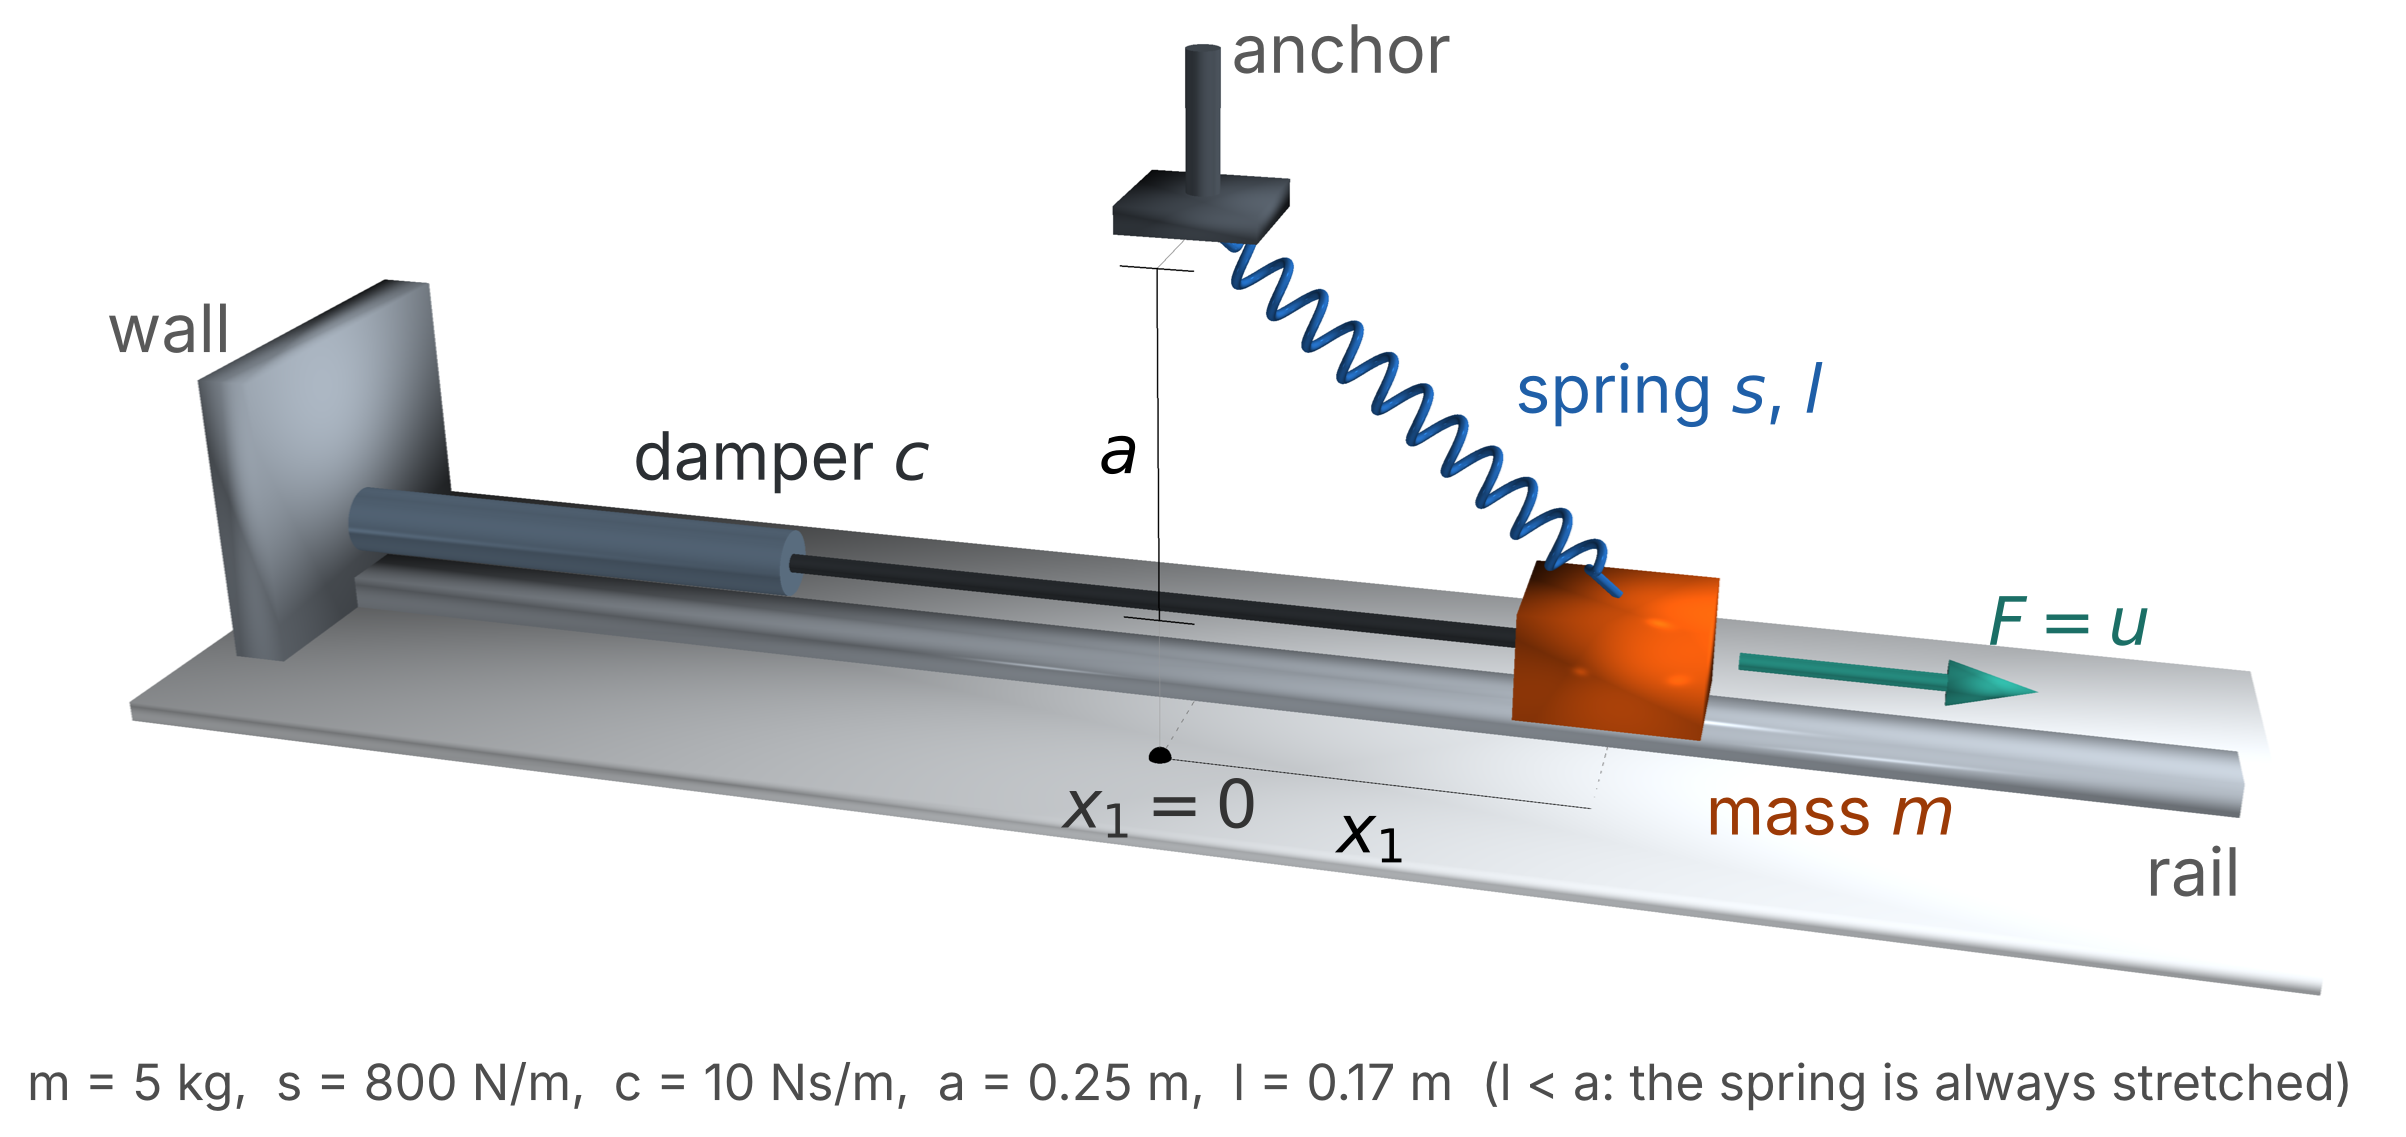
\includegraphics[width=\textwidth]{fig_system_3d.png}\\[-1pt]{\small (a)}
\end{minipage}\hfill
\begin{minipage}[c]{0.45\textwidth}\centering\footnotesize
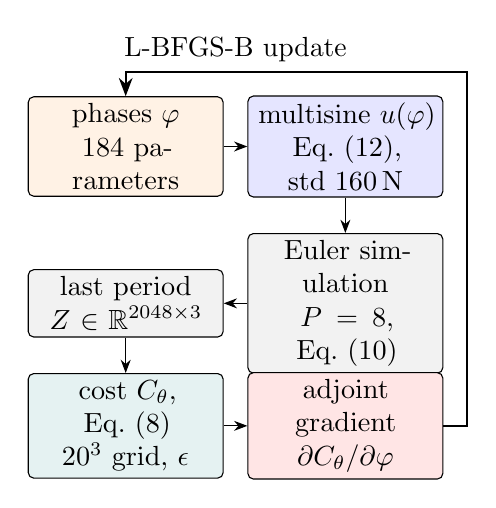
\begin{tikzpicture}[node distance=4.5mm and 3mm,>=Stealth,
  b/.style={draw,rounded corners=2pt,align=center,inner sep=2.5pt,minimum height=8mm,text width=23mm,fill=#1!10},
  b/.default=gray]
\node[b=orange] (ph) {phases $\varphi$\\184 parameters};
\node[b=blue,right=of ph] (u) {multisine $u(\varphi)$\\Eq.~(12), std 160\,N};
\node[b=gray,below=of u] (sim) {Euler simulation\\$P=8$, Eq.~(10)};
\node[b=gray,left=of sim] (z) {last period\\$Z\in\mathbb R^{2048\times3}$};
\node[b=teal,below=of z] (c) {cost $C_\theta$, Eq.~(8)\\$20^3$ grid, $\epsilon$};
\node[b=red,right=of c] (g) {adjoint gradient\\$\partial C_\theta/\partial\varphi$};
\draw[->] (ph)--(u); \draw[->] (u)--(sim); \draw[->] (sim)--(z); \draw[->] (z)--(c); \draw[->] (c)--(g);
\draw[->,thick] (g.east) -- ++(3mm,0) |- ([yshift=3mm]u.north) -| node[pos=0.25,above]{L-BFGS-B update} (ph.north);
\end{tikzpicture}\\[1pt]{\small (b)}
\end{minipage}
\caption{(a) Test system of Sec.~4.1 of the paper, drawn to scale for $a$ and $l$ (own 3-D rendering): the
spring is anchored a height $a$ above the cart, so its horizontal restoring force
$s\,x_1(1-l/\sqrt{x_1^2+a^2})$ is nonlinear in $x_1$. (b) The reproduced optimisation loop: only the phases
change, the amplitude spectrum and the signal power stay fixed.}
\label{fig:sys}\end{figure*}

\section{Reproduction Protocol}
\textbf{Implementation.} All code is my own Python 3.13 (NumPy 2.5.3, SciPy 1.18.1, Matplotlib 3.11.2;
Numba 0.68.1 for the extension); the authors released none. CPU only, float64.
The gradient $\partial C_\theta/\partial\varphi$ is exact: Eq.~\eqref{eq:cost} is differentiated in closed
form and the chain rule is run backwards through the Euler recursion (an adjoint, \mEvalTime\,s per cost+gradient)
and through the multisine. It matches central differences to \mGradErr{} of $\max|g|$. Phases are
optimised with L-BFGS-B \citep{Byrd1995} (max.\ 1000 iterations, $f_{tol}=10^{-10}$, $g_{tol}=10^{-6}$).

\begin{table}[t]\centering\footnotesize\setlength{\tabcolsep}{2.5pt}
\caption{Result map: each published target, the script that regenerates it, the comparison metric and
the final status.}\label{tab:map}
\begin{tabular}{@{}lllc@{}}\toprule
ID & Paper item & Metric (script \texttt{run\_*}) & Status\\\midrule
T1 & Fig.~3 & spectrum, CF (\texttt{sec44}) & R\\
T2 & Sec.~4.4 & $C_{init},C_{opt}$, ratio (\texttt{sec44}, \texttt{h1\_fmincon}) & P\\
T3 & Fig.~4 & $\kappa$, share in $\Dz$ (\texttt{sec44}) & R\\
T4 & Fig.~5 & 3-D view, $\kappa$ (\texttt{sec44}) & R\\
T5 & Fig.~6 & samples per $u$-bin (\texttt{sec44}) & R\\
T6 & Sec.~4.5, Fig.~7 & CF, $C_\theta$ (\texttt{sec45}) & R/P\\
T7 & Sec.~4.6, Fig.~8 & box-plot statistics (\texttt{mc\_phases}) & P\\
\bottomrule\multicolumn{4}{@{}l}{\scriptsize R: reproduced, P: partially (\S\ref{sec:h1}). T4: Fig.~\ref{fig:3d}.}
\end{tabular}\end{table}

\begin{table}[t]\centering\footnotesize\setlength{\tabcolsep}{3pt}
\caption{Settings. Top: given in the paper. Bottom: not reported, fixed in the M2 protocol before any result.}
\label{tab:set}\begin{tabular}{@{}ll@{}}\toprule
$m,s,a,l,c$ & 5\,kg, 800\,N/m, 0.25\,m, 0.17\,m, 10\,Ns/m\\
$T_s$, $N$, lines & 0.01\,s, 2048, $l=21\ldots204$ (1.03--9.96\,Hz)\\
$\Dz$, grid, $\Sigma$ & $\pm400$\,N$\times\pm2$\,m$\times\pm20$\,m/s, $20^3$, diag$(40^2,0.2^2,2^2)$\\\midrule
$\epsilon$ & $10^{-3}$ (paper's 287.15 implies $\epsilon\le3.5\times10^{-3}$)\\
Steady state & from rest, keep period $P=\nP$, tolerance $10^{-6}$\\
Optimiser & L-BFGS-B, $\le$1000 it., $f_{tol}=10^{-10}$, $g_{tol}=10^{-6}$\\
Seeds & 0 (T1--T6), 1--20 (T7), \texttt{numpy.default\_rng}\\
Schroeder & $\varphi_l=-l(l-1)\pi/184$, $l=1\ldots184$\\
\bottomrule\end{tabular}\end{table}

\textbf{Settings not reported in the paper} (fixed in M2 before any result):
$\epsilon=10^{-3}$ (the published 287.15 requires $\epsilon\le3.5\times10^{-3}$ since $C_\theta\le1/\epsilon$);
start from rest and keep period $P=8$ (steady state checked by a period-to-period criterion $10^{-6}$);
seeds 0 (T1--T6) and 1--20 (T7) with \texttt{numpy.default\_rng}; Schroeder phases
$\varphi_l=-l(l-1)\pi/184$, $l=1\ldots184$.

\textbf{Deviations.} (i) \texttt{fmincon}$\to$L-BFGS-B (both gradient-based local methods; tested in
\S\ref{sec:h1}); (ii) PyTorch autograd$\to$hand-derived adjoint (PyTorch was not installable at M3);
(iii) $P=5\to8$: the first seed-0 optimum violated the steady-state rule at $P=5$, so all runs were repeated.

\textbf{Data split and validation.} No model is fitted in Secs.~4.4--4.6, so there is no estimation/validation split.
Instead: 20 independent seeds, re-evaluation on an independent $30^3$ grid
(\nGridInit$\to$\nGridOpt, ratio \nGridRatio), a different initial state (state difference
\nXzeroOpt) and $P=12$ (\nPtenOpt), plus eight unit checks D1--D8 (dimensions, free decay, steady state,
kernel, cost bound, gradient, Euler stability, grid), all passed. The 20 Monte-Carlo optimisations were rerun for M4:
the \mRerunIdentical{} runs on the M3 machine reproduced the M3 optima bit for bit; the runs on a second
machine (Windows, other BLAS) agree to $\le$\mRerunItTwentyMax{} after 20 iterations, but round-off
differences grow along the non-convex optimisation path and the converged costs differ by up to
\mRerunFinalMax\,\% (median \mRerunFinalMed\,\%).

\begin{table}[t]\centering\footnotesize\setlength{\tabcolsep}{3pt}
\caption{Verification and validation checks (all pass).}\label{tab:diag}
\begin{tabular}{@{}lll@{}}\toprule
ID & Check & Result\\\midrule
D1 & input dimension, mean, std, lines & std 160.000\,N, 184 lines\\
D2 & free decay from $x_1=0.5$\,m & stable, damped\\
D3 & steady state at $P=\nP$ & rel.\ change \nSSrelOpt\\
D4/D5 & kernel $=1$ at $z_k=\tilde z_i$; $C\le1/\epsilon$ & exact\\
D6 & adjoint vs.\ central differences & $\le$\mGradErr$\,\max|g|$\\
D7 & Euler spectral radius & \mRadZero{} / \mRadTwo{} $<1$\\
D8 & grid spacings & equal to paper\\
V2 & independent $30^3$ grid & ratio \nGridRatio\\
V3/V4 & other $x_0$; $P=12$ & \nXzeroOpt{} / \nPtenOpt\\
V6 & rerun of 20 MC runs & same machine: identical\\
\bottomrule\end{tabular}\end{table}

\section{Reproduction Results}
\begin{table}[t]\centering\scriptsize
\caption{Published vs.\ reproduced values (seed 0 unless stated; MC = 20 seeds, median [min--max]).
Rows ``20 it.'' and ``MC initial'' are from the M3 runs (\texttt{results/mc}); rows ``full'', ``BFGS-FD'' and
the MC crest factor from the M4 runs (\texttt{results/mc\_phases}, \texttt{h1\_fmincon}).}
\label{tab:comp}\setlength{\tabcolsep}{2pt}
\begin{tabular}{@{}lll@{}}\toprule
Quantity & Paper & Reproduced\\\midrule
$C_\theta$ initial (seed 0) & 287.15 & \nCinit{} ($\nRelCinit\,\%$)\\
$C_\theta$ initial, MC & $\approx$268 & \nMCiMedian{} [\nMCiMin--\nMCiMax]\\
$C_\theta$ optimised, full run & 3.88 & \nCopt{} (\nNit{} it.)\\
$C_\theta$ after 16 / 20 it. & 3.88 & \nEaC{} / \nEbC\\
Ratio $C_{init}/C_{opt}$ & 69 (text), 74.0 & \nRatio{} (full); \nEbR{} (20 it.)\\
MC final $C_\theta$, 20 it. & $\approx$3.65 [2.9--5.5] & \nMCtMedian{} [\nMCtMin--\nMCtMax]\\
MC final $C_\theta$, full & -- & \mCfullMed{} [\mCfullMin--\mCfullMax]\\
MC final $C_\theta$, BFGS-FD & -- & \mHoneMed{} [\mHoneMin--\mHoneMax]\\
CF Schroeder & 1.87 & \nCFschA{} (+\nRelCFsch\,\%)\\
CF optimised & 3.67 & \nCFopt; MC 20 it.\ \mCFtwentyMed{} [\mCFtwentyMin--\mCFtwentyMax]\\
Coverage $\kappa$ rand./Sch./opt. & -- & \nKapInit{} / \nKapSch{} / \nKapOpt{}\,\%\\
\bottomrule\end{tabular}\end{table}

\begin{figure}[t]\centering
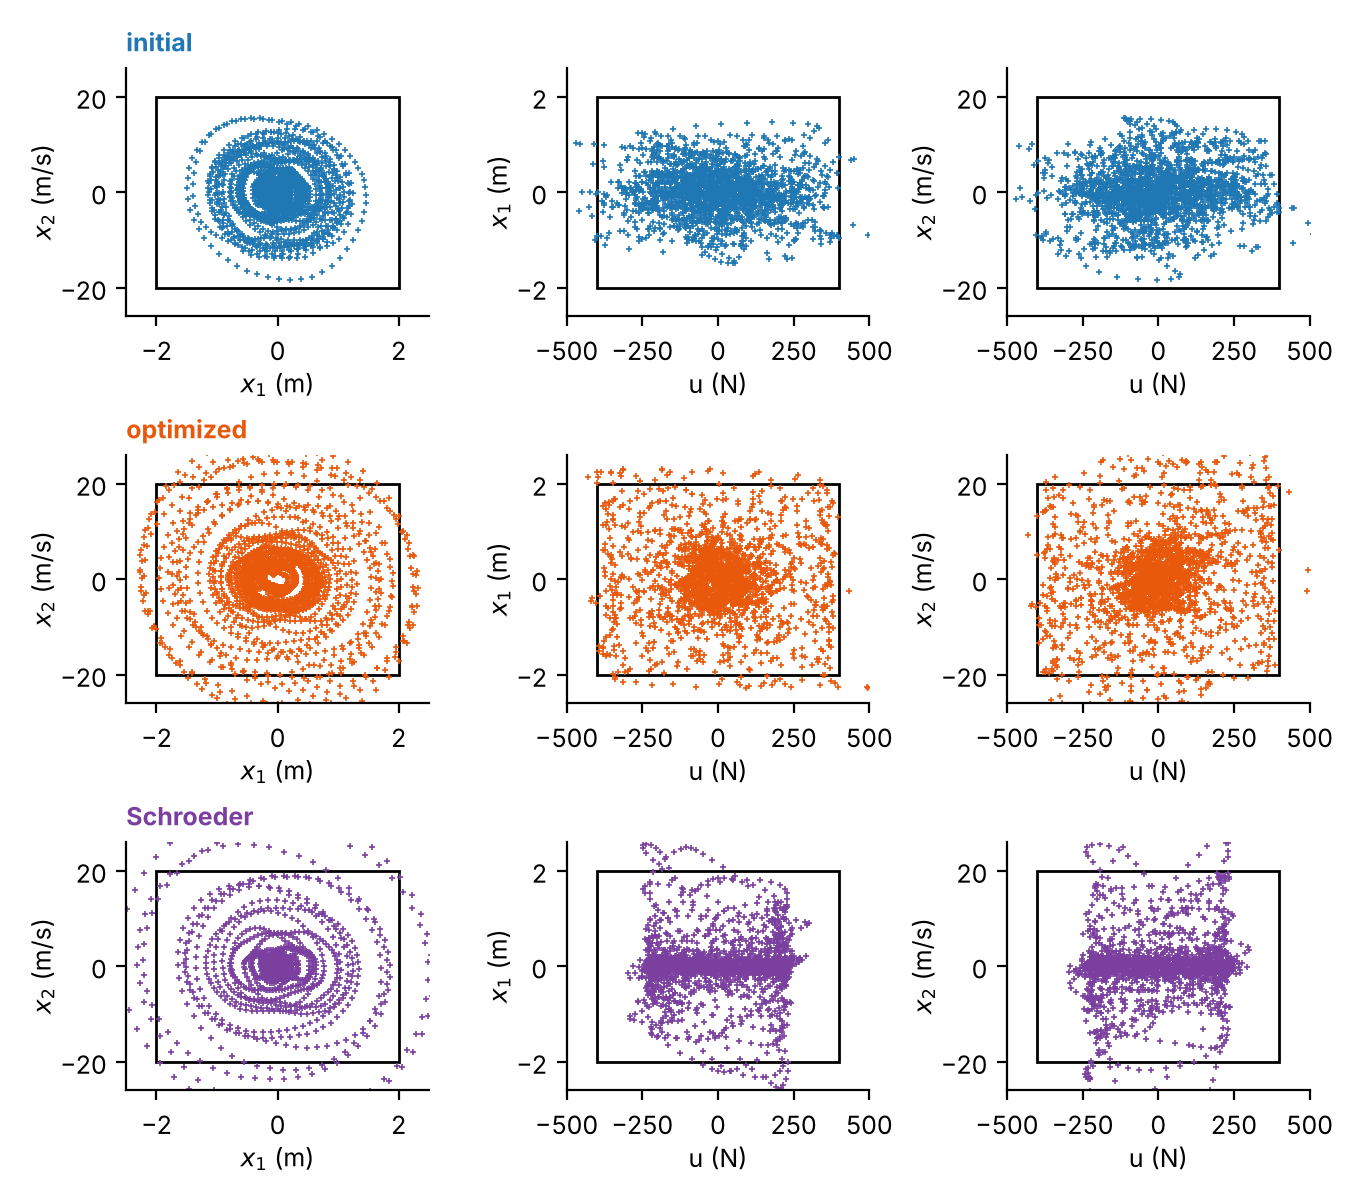
\includegraphics[width=\columnwidth]{fig4_side_views.png}
\caption{T3: input--state samples of the initial (blue), optimised (orange) and Schroeder (purple) signals,
seed 0; boxes are the borders of $\Dz$. As in Fig.~4 of the paper, the optimised data spread towards the
borders, mostly along $u$, while the Schroeder data stay inside $|u|\lesssim300$\,N.}
\label{fig:side}\end{figure}

\begin{figure}[t]\centering
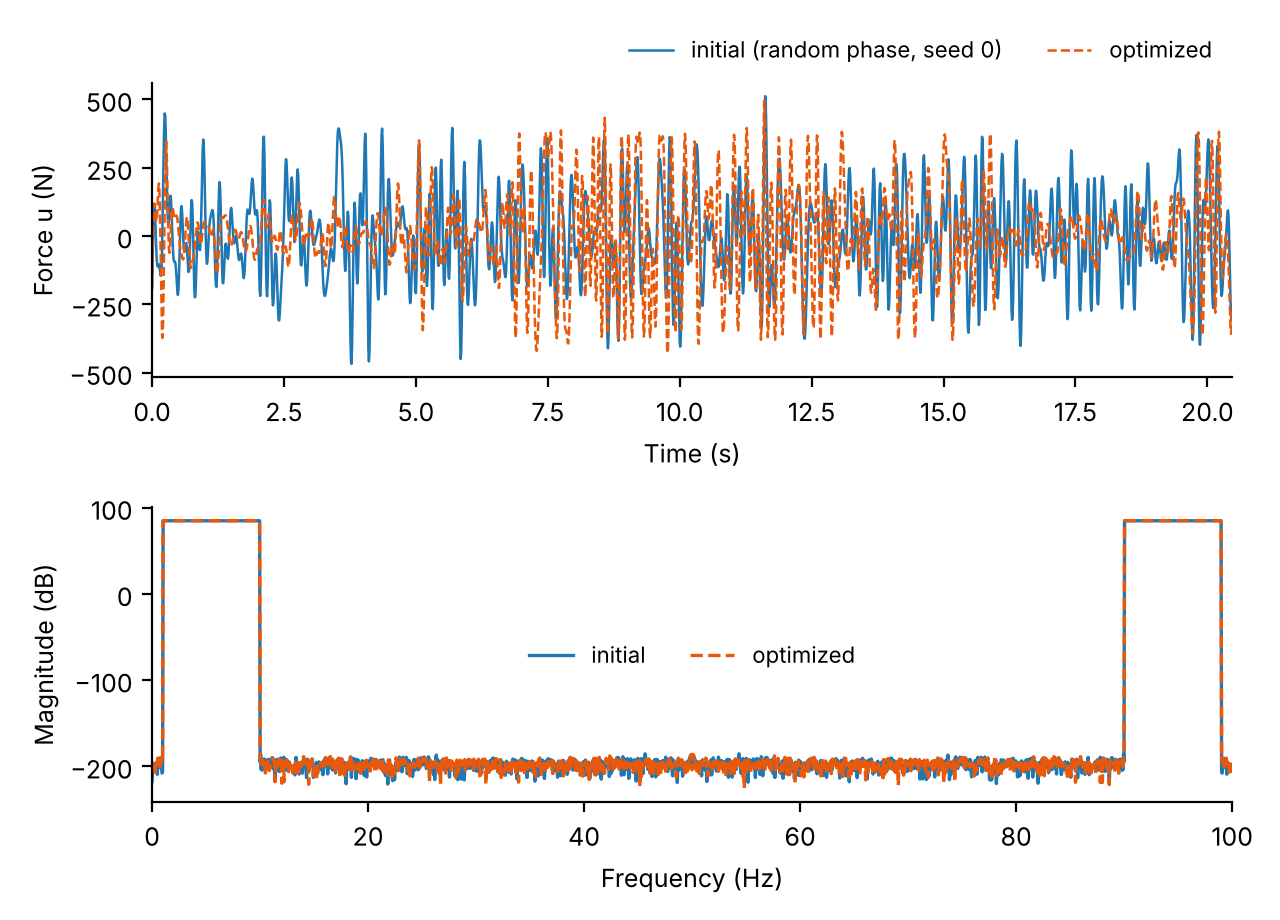
\includegraphics[width=\columnwidth]{fig3_signal.png}
\caption{T1: initial (blue) and optimised (orange) multisine, seed 0, in time and frequency (two-sided
$|$DFT$|$ over 0--100\,Hz, the paper's convention; 90--99\,Hz is the mirror image). The amplitude
spectrum is identical (\mLineDB\,dB on lines 21--204); only the waveform changes.}
\label{fig:sig}\end{figure}

\begin{figure*}[t]\centering
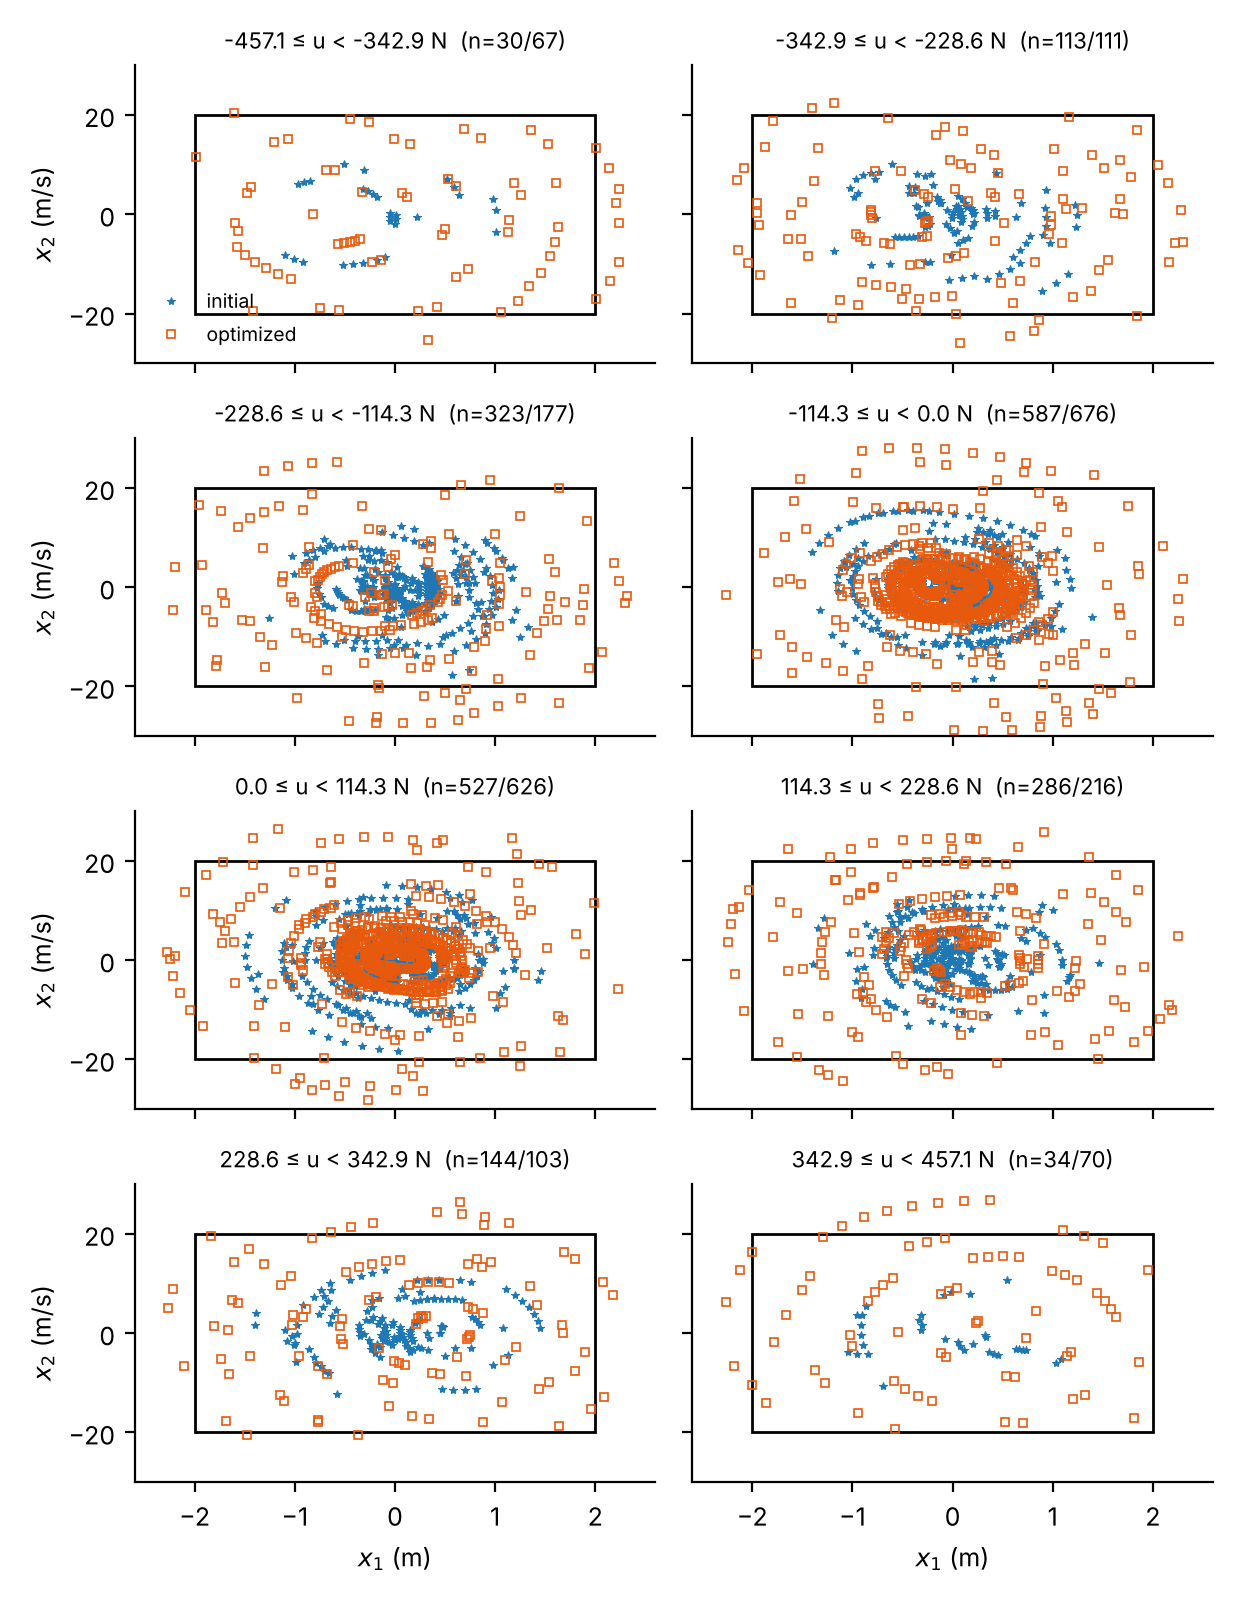
\includegraphics[width=0.44\textwidth]{fig6_slices.png}\hfill
\begin{minipage}[b]{0.54\textwidth}\centering
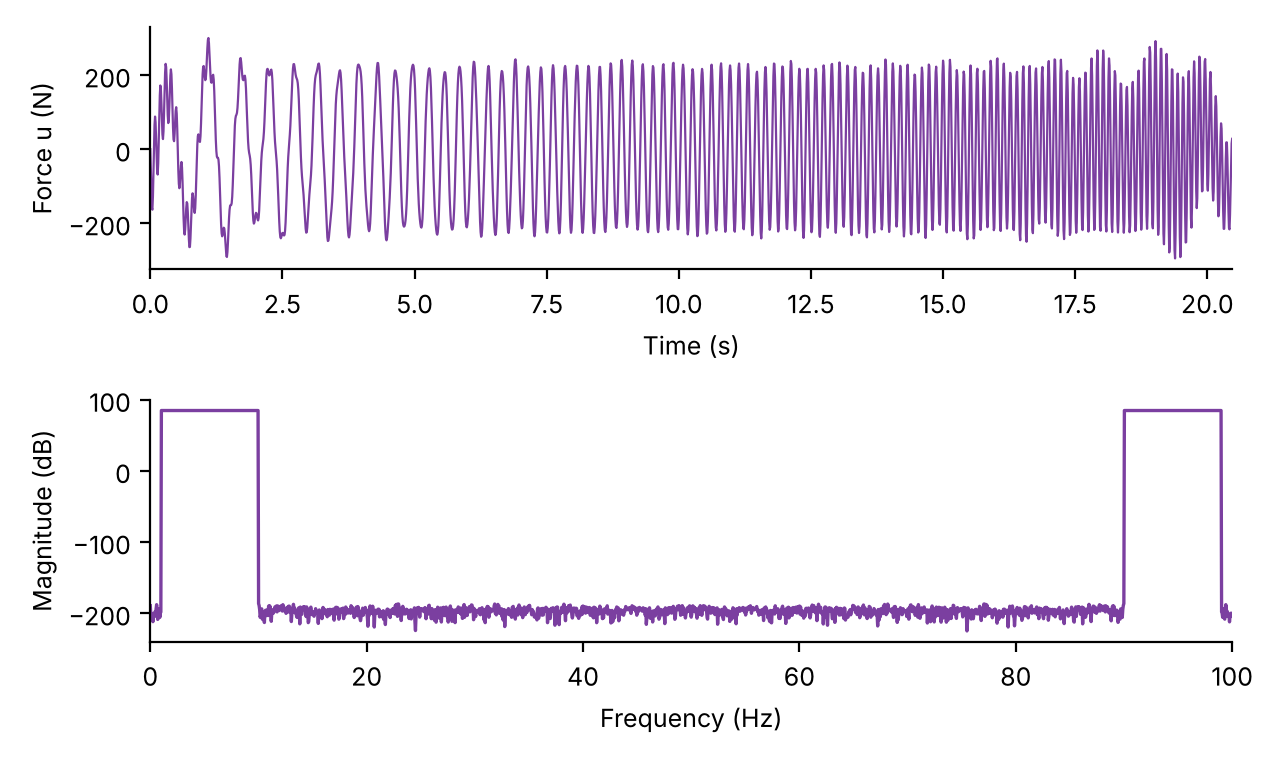
\includegraphics[width=\textwidth]{fig7_schroeder.png}\\[4pt]
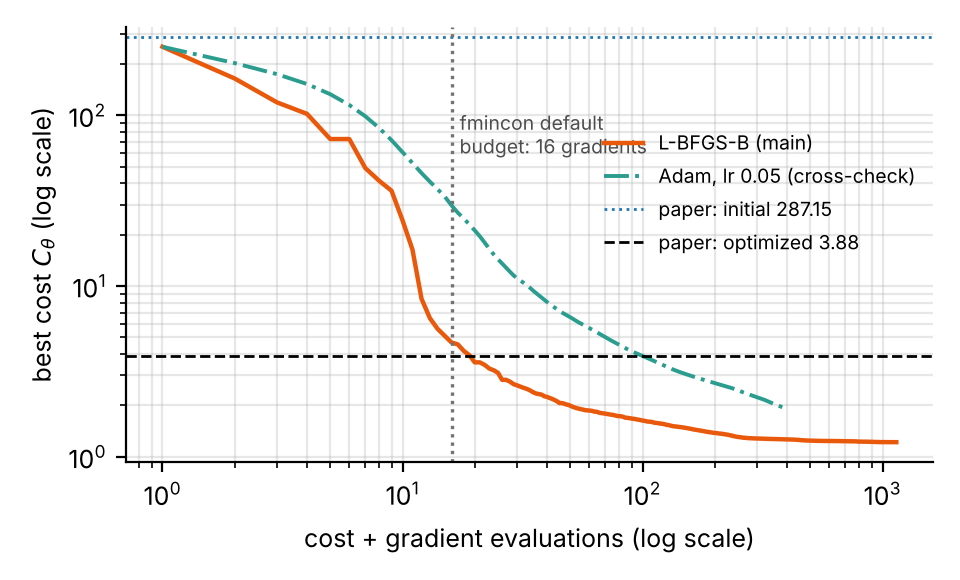
\includegraphics[width=0.78\textwidth]{fig_cost_history.png}
\end{minipage}
\caption{Left, T5: eight $x_1$--$x_2$ slices along $u$ (paper Fig.~6), initial (blue) vs.\ optimised
(orange), seed 0; the outer slices are almost empty for the random-phase input. Top right, T6: Schroeder
multisine (paper Fig.~7). Bottom right: cost vs.\ evaluations for seed 0 (L-BFGS-B and the Adam cross-check);
the paper's 3.88 is passed after \nFirstBelow{} L-BFGS-B iterations (about 20 evaluations).}
\label{fig:t56}\end{figure*}

\begin{figure}[t]\centering
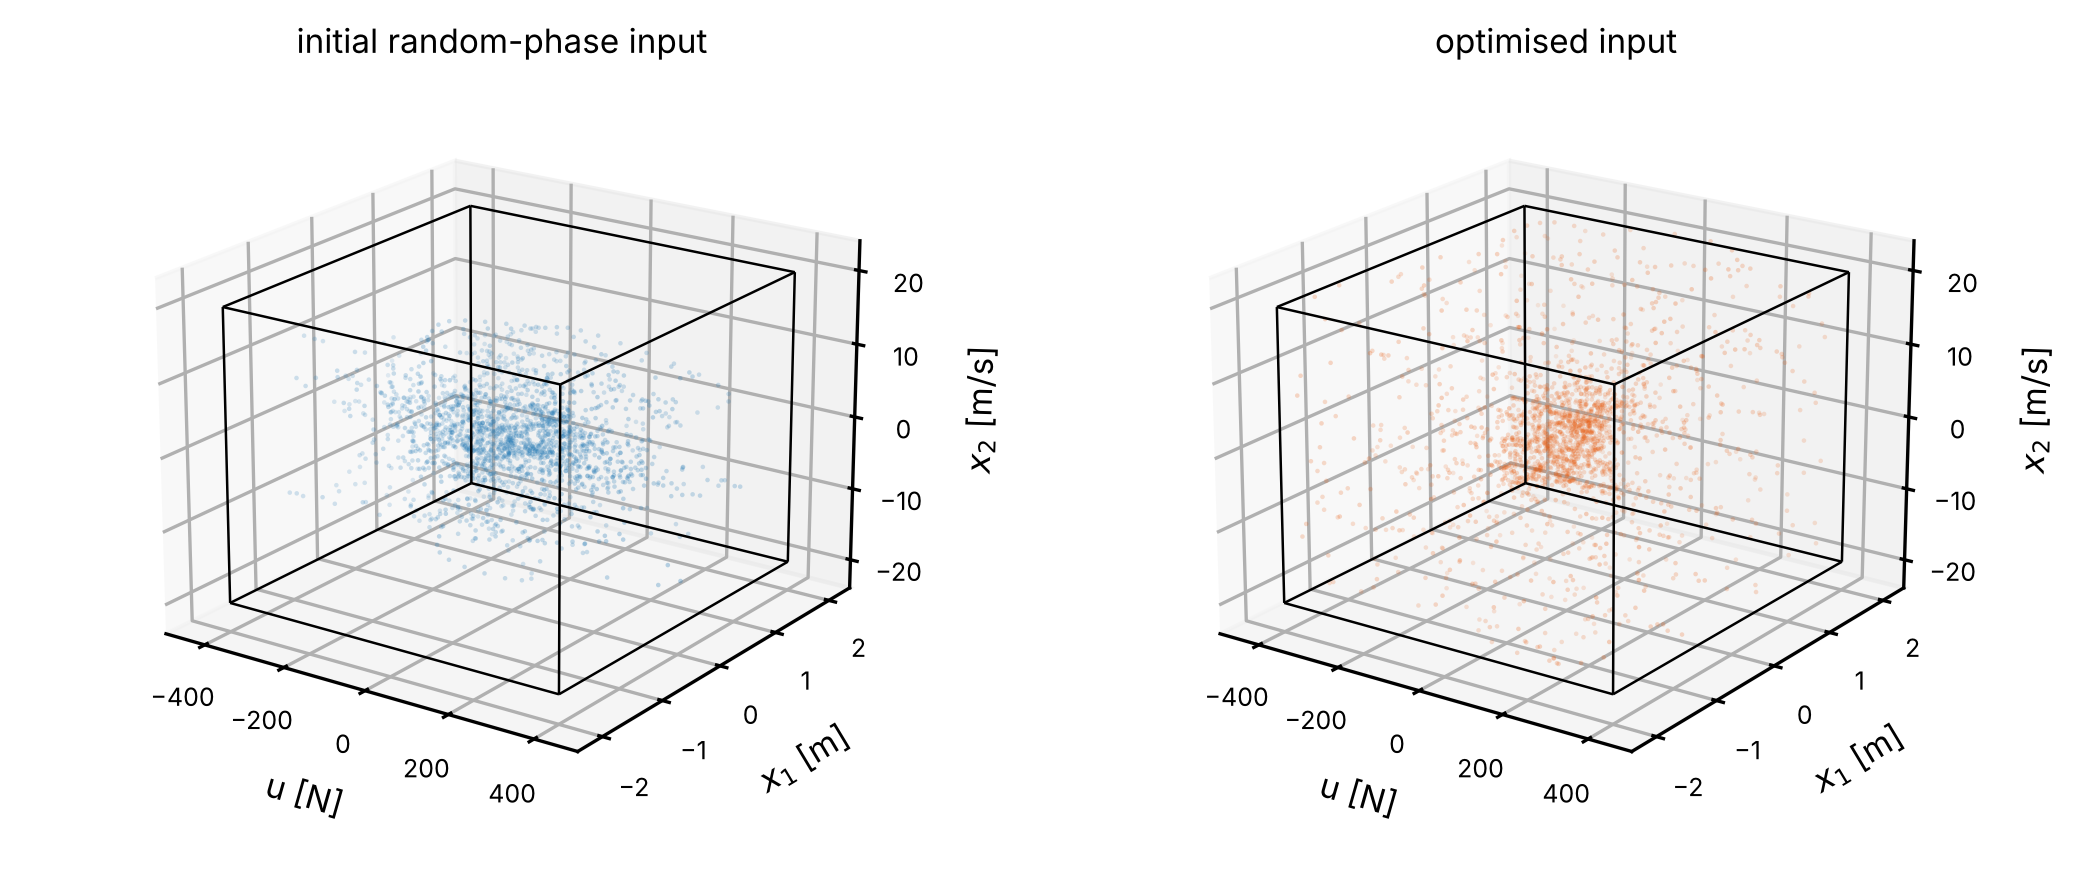
\includegraphics[width=\columnwidth]{fig_states_3d.png}
\caption{T4: 3-D view of the 2048 input--state samples of seed 0 inside $\Dz$ (black box), paper Fig.~5.
The random-phase samples form a cloud in the centre; the optimised samples reach the faces and corners of the
box, with a dense core remaining.}
\label{fig:3d}\end{figure}

\textbf{T1, T3--T5 (signal and coverage).} The optimised signal keeps the amplitude spectrum to
$\max_l|\Delta A_l|=\ndA$\,N, while the waveform changes (crest factor \nCFinit$\to$\nCFopt).
The three qualitative findings of the paper's Figs.~4--6 are reproduced (Fig.~\ref{fig:side}): the
random-phase data cluster in the centre, the optimised data fill the box, and the Schroeder data spread in
$x_1,x_2$ but not along $u$. Quantitatively, the share of grid points with $d_i\ge1$ rises from
\nKapInit\,\% to \nKapOpt\,\% and the two outer $u$-slices of Fig.~6 receive \nBinLoOpt{} and \nBinHiOpt{}
samples instead of \nBinLoInit{} and \nBinHiInit.

\textbf{T6 (Schroeder).} CF\,=\,\nCFschA{} vs.\ 1.87 (+\nRelCFsch\,\%); the index convention
$l=21\ldots204$ gives \nCFschB. Every optimised signal has a lower cost than Schroeder (\nCsch; \mNOptBelowSch/20
seeds), and Schroeder is below the random-phase signal for \mNSchBelowRand/20 seeds (random-phase costs range
\nMCiMin--\nMCiMax). The optimised CF depends on how far the optimisation goes: \mCFsixteenMed{} after 16 and
\mCFtwentyMed{} after 20 iterations (medians over 20 seeds) vs.\ 3.67 published, and \mCFfullMed{} at the
end, so the published value lies inside our early-stopped range [\mCFsixteenMin--\mCFsixteenMax].

\subsection{T2 and T7: the optimised cost, and hypothesis H1}\label{sec:h1}
The initial costs agree (seed 0: \nRelCinit\,\%; our 20-seed range contains 287.15), which confirms the
grid, kernel and $\epsilon$. The optimised cost does not: L-BFGS-B passes 3.88 after a median of
\mItPaperMed{} iterations and keeps going to \mCfullMed. \textbf{Hypothesis H1}: the authors stopped early. With
default options, \texttt{fmincon} uses forward finite differences (185 evaluations per gradient) and
\texttt{MaxFunctionEvaluations}\,=\,3000, i.e.\ about 16 gradients. M3 tested H1 only by stopping our
L-BFGS-B early. For M4 we ran an \emph{fmincon-like} optimiser: dense BFGS with forward-difference
gradients and a hard cap of 3000 cost evaluations, no exact gradient (seeds \mHoneSeeds; \mHoneTime\,min
each). It ends at a median of \mHoneMed{} [IQR \mHoneQOne--\mHoneQThree, range \mHoneMin--\mHoneMax] versus
the paper's $\approx$3.65 [2.9--5.5] (Fig.~\ref{fig:h1}). The fmincon-like runs overlap the published
box but are more spread (\mHoneAbove{} of the 10 runs end above the paper's maximum of 5.5), while the 20-iteration L-BFGS-B runs (median \nMCtMedian) match the published
median closely, and converged runs end about three times lower. A budget-limited quasi-Newton run
therefore stops in the paper's cost range, and a converged one does not. This is consistent with early
stopping (H1), but our fmincon-like emulation is more spread than the published box, so the authors' exact
budget or algorithm (interior-point) is not identified; H1 remains a plausible explanation, not a proven one.
The close match of the 20-iteration median was found at one of three stopping points we tried (16/20/25).

\begin{figure}[t]\centering
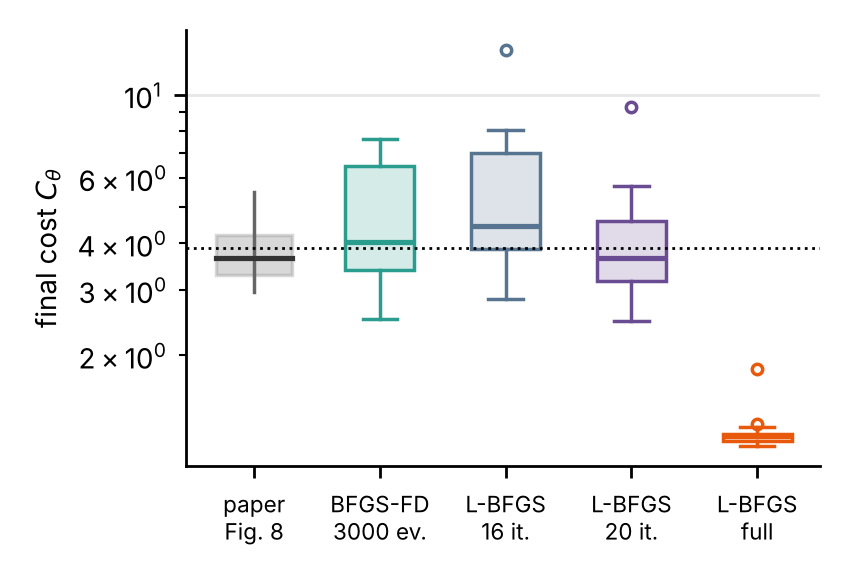
\includegraphics[width=0.94\columnwidth]{fig_h1.png}
\caption{T7 and H1: final costs. Grey: paper Fig.~8 (read from the axes). Teal: fmincon-like BFGS with
forward differences, 3000 evaluations (10 seeds, 0--9; seed 0 is not in the L-BFGS-B set). Blue/purple/orange: our L-BFGS-B runs (seeds 1--20) after 16 and 20
iterations and at convergence. Dotted: published 3.88.}
\label{fig:h1}\end{figure}

\textbf{$\epsilon$ with re-optimisation.} Re-optimising seed 0 for $\epsilon\in\{10^{-4},10^{-3},
3{\cdot}10^{-3},10^{-2}\}$ (300 iterations) changes the initial cost strongly
(\mEpsAInit, \mEpsBInit, \mEpsCInit, \mEpsDInit) but the designed signal hardly: evaluated with the common
$\epsilon=10^{-3}$, the optima cost \mEpsACref, \mEpsBCref, \mEpsCCref, \mEpsDCref{} and cover
\mEpsKapMin--\mEpsKapMax\,\% of the grid (Table~\ref{tab:eps}). Only $\epsilon\approx10^{-3}$ reproduces the published initial cost,
so $\epsilon$ explains the absolute values but not the gap in $C_{opt}$.

\begin{table}[t]\centering\footnotesize\setlength{\tabcolsep}{3pt}
\caption{$\epsilon$ sensitivity with re-optimisation (seed 0, 300 iterations). $C^{(10^{-3})}_{opt}$: optimum
evaluated with the common $\epsilon=10^{-3}$.}\label{tab:eps}
\begin{tabular}{@{}lrrrrr@{}}\toprule
$\epsilon$ & $C_{init}$ & $C_{opt}$ & ratio & $C^{(10^{-3})}_{opt}$ & $\kappa$ [\%]\\\midrule
$10^{-4}$ & \mEpsAInit & \mEpsAOpt & \mEpsARatio & \mEpsACref & \mEpsAKap\\
$10^{-3}$ & \mEpsBInit & \mEpsBOpt & \mEpsBRatio & \mEpsBCref & \mEpsBKap\\
$3\cdot10^{-3}$ & \mEpsCInit & \mEpsCOpt & \mEpsCRatio & \mEpsCCref & \mEpsCKap\\
$10^{-2}$ & \mEpsDInit & \mEpsDOpt & \mEpsDRatio & \mEpsDCref & \mEpsDKap\\
\bottomrule\end{tabular}\end{table}

\textbf{Reproduction status.} T1, T3, T4, T5: reproduced. T6: Schroeder CF reproduced (0.5\,\%), optimised
CF partially (depends on the stopping point). T2, T7: \emph{partially reproduced}: the initial costs, the
ranking and the early-stopped values match; the converged values are lower, consistent with H1. The paper's
``69$\times$'' is inconsistent with its own numbers ($287.15/3.88=74.0$).

\section{Extension: From Coverage to Model Accuracy}
% Extension section (bonus). All numbers are macros from ../results/numbers_m4.tex.
\textbf{Question and hypotheses.} The paper motivates the cost~\eqref{eq:cost} by model quality but never
identifies a model. We test three hypotheses on the reproduced designs:
\textbf{E1} a model identified from the optimised input is more accurate over $\Dz$ than one identified
from a random-phase or Schroeder input with the same amplitude spectrum;
\textbf{E2} the gain survives when the design is computed on a model \emph{identified} from a first
random-phase experiment instead of the true system (the realistic case: the system to be identified is
unknown);
\textbf{E3} the space-filling cost is a useful predictor of model error.

\begin{figure}[t]\centering\footnotesize
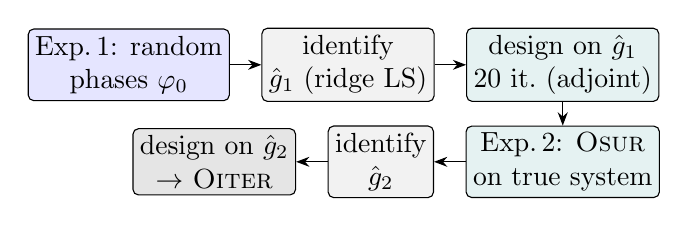
\begin{tikzpicture}[node distance=3mm and 4mm,>=Stealth,
  b/.style={draw,rounded corners=2pt,align=center,inner sep=2.5pt,minimum height=7mm,fill=#1!10},b/.default=gray]
\node[b=blue] (r) {Exp.\,1: random\\phases $\varphi_0$};
\node[b=gray,right=of r] (id1) {identify\\$\hat g_1$ (ridge LS)};
\node[b=teal,right=of id1] (d1) {design on $\hat g_1$\\20 it.\ (adjoint)};
\node[b=teal,below=of d1] (e2) {Exp.\,2: \st{Osur}\\on true system};
\node[b=gray,left=of e2] (id2) {identify\\$\hat g_2$};
\node[b=black,left=of id2] (d2) {design on $\hat g_2$\\$\to$ \st{Oiter}};
\draw[->] (r)--(id1); \draw[->] (id1)--(d1); \draw[->] (d1)--(e2); \draw[->] (e2)--(id2); \draw[->] (id2)--(d2);
\end{tikzpicture}
\caption{Surrogate-in-the-loop design (E2): the true system is only used to run experiments; every design
step uses an identified model.}\label{fig:loop}\end{figure}

\textbf{Controlled design.} Only the phases differ between designs; spectrum (184 lines, std 160\,N),
length ($N=2048$, one steady-state period), model class, estimator and noise are identical.
Eight designs per seed $s=1\ldots20$: \st{R} random phases $\varphi_0(s)$; \st{S} Schroeder;
\st{O16}, \st{O20}, \st{Ofull}: the reproduced L-BFGS-B runs on the true system after 16, 20 and
$\le$1000 iterations; \st{Osur}: 20 iterations from $\varphi_0(s)$ on the model identified from the
\st{R} experiment, with the exact adjoint gradient propagated through the identified model;
\st{Oiter}: the model is re-identified from the \st{Osur} experiment and the design continued for 20
iterations (two-round sequential design, cf.\ \citealp{Pronzato2013}); \st{Osur100}: 100 iterations
on the first surrogate (40\,dB only).
\emph{Measurement}: both states are measured with white Gaussian sensor noise of \emph{fixed absolute}
level (a sensor does not know the input), set to 40 or 30\,dB below the state variance of the reference
random-phase signal, plus a noise-free case; the noise sequence of a seed is shared by all designs.
\emph{Model}: the kinematics $x_{1,k+1}=x_{1,k}+T_sx_{2,k}$ are known; the force law is a black box
$x_{2,k+1}=x_{2,k}+T_s\,\theta^\top\phi(z_k)$, with $\phi$ = constant, linear terms and 343 Gaussian
radial basis functions on a $7^3$ grid over $\Dz$ (width = spacing). RBFs are local, so they learn only
where data exist. \emph{Estimator}: ridge least squares on the one-step data,
$\hat\theta=(\Phi^\top\Phi+\lambda N I)^{-1}\Phi^\top y$, with $\lambda$ chosen by 5-fold blocked
cross-validation on the training data only \citep{Ljung1999}.
\emph{Tests} (never used for fitting or tuning): $e_{\mathrm{uni}}$, the NRMSE of $\hat g$ on 20\,000
points drawn uniformly in $\Dz$ (the region the user asked to model); $e_{\mathrm{sim}}$, the free-run
simulation NRMSE of $(x_1,x_2)$ on five new random-phase multisines at the design level (std 160\,N) and
at 1.5$\times$ that level (240\,N, stress test). \emph{Statistics}: medians over the 20 paired seeds and
a one-sided paired Wilcoxon signed-rank test against \st{R} \citep{Wilcoxon1945}, with a diverged simulation
ranked as the worst result. The $p$-values are unadjusted; all \mNTests{} tests are listed in the package,
and every $e_{\mathrm{uni}}$ improvement also survives a Bonferroni correction (all $p\le\mMaxPeuni$).
The two test types favour different designs: $e_{\mathrm{uni}}$ weights all of $\Dz$ equally, including
state combinations a random-phase input rarely reaches, while the random-phase free-run tests at 160\,N live
where random-phase training data are dense.

\begin{table}[t]\centering\scriptsize\setlength{\tabcolsep}{2.6pt}
\caption{Extension results, medians over \mNExt{} seeds. $^*$: better than random, $^\circ$: worse
than random (paired Wilcoxon, $p<0.01$); $^\dagger$: some free-run simulations diverged (counted as
failures). $C_\theta,\kappa$: coverage achieved on the true system.}
\label{tab:ext}% generated by m4_analysis.py
\begin{tabular}{@{}lrrrrrrr@{}}\toprule
 & \multicolumn{3}{c}{$e_{\mathrm{uni}}$ [\%]} & \multicolumn{2}{c}{$e_{\mathrm{sim}}$ [\%], 40 dB} & & \\
\cmidrule(lr){2-4}\cmidrule(lr){5-6}
Design & clean & 40\,dB & 30\,dB & 160\,N & 240\,N & $C_\theta$ & $\kappa$[\%]\\\midrule
random & 19.0 & 19.0 & 22.2 & 17.7 & 107.6$^\dagger$ & 251 & 37\\
Schroeder & 9.8$^{*}$ & 11.8$^{*}$ & 5.6$^{*}$ & 40.5$^{\circ}$ & 49.9$^{*}$ & 159 & 35\\
opt. 16 it. & 2.2$^{*}$ & 2.7$^{*}$ & 4.3$^{*}$ & 22.5 & 12.6$^{*}$ & 4.45 & 48\\
opt. 20 it. & 2.2$^{*}$ & 2.6$^{*}$ & 4.0$^{*}$ & 22.0 & 12.7$^{*}$ & 3.65 & 49\\
opt. full & 1.7$^{*}$ & 2.2$^{*}$ & 3.6$^{*}$ & 23.6 & 12.9$^{*}$ & 1.21 & 60\\
surrogate & 2.9$^{*}$ & 4.3$^{*}$ & 6.5$^{*}$ & 18.4 & 16.8$^\dagger$$^{*}$ & 46.6 & 45\\
iterative & 2.1$^{*}$ & 2.7$^{*}$ & 4.3$^{*}$ & 23.3$^{\circ}$ & 13.1$^{*}$ & 7.08 & 51\\
surr. 100 it. & -- & 3.7$^{*}$ & -- & 20.0 & 16.2$^\dagger$$^{*}$ & 42.7 & 47\\
\bottomrule\end{tabular}
\end{table}

\begin{figure*}[t]\centering
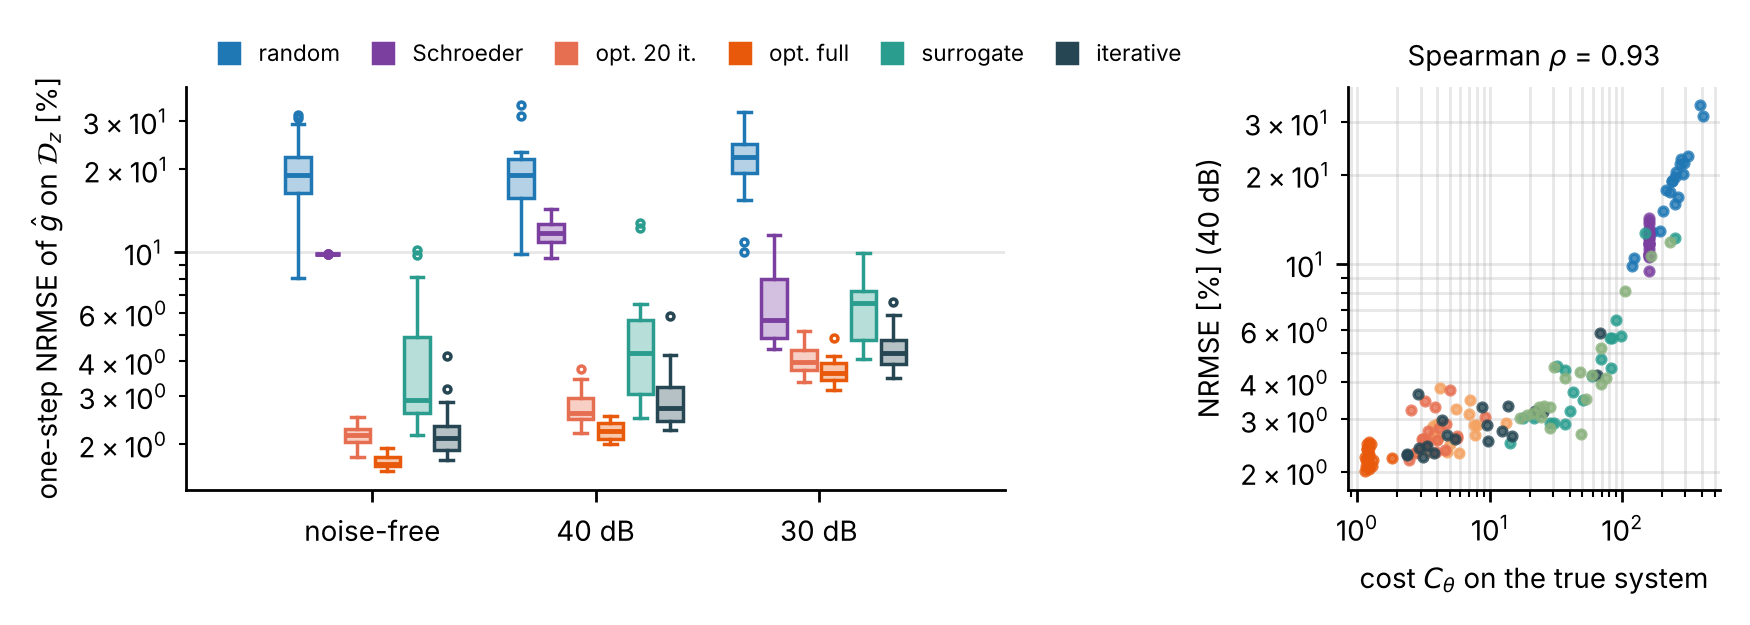
\includegraphics[width=0.85\textwidth]{fig_ext_accuracy.png}\\[2pt]
\small (a)\\[2pt]
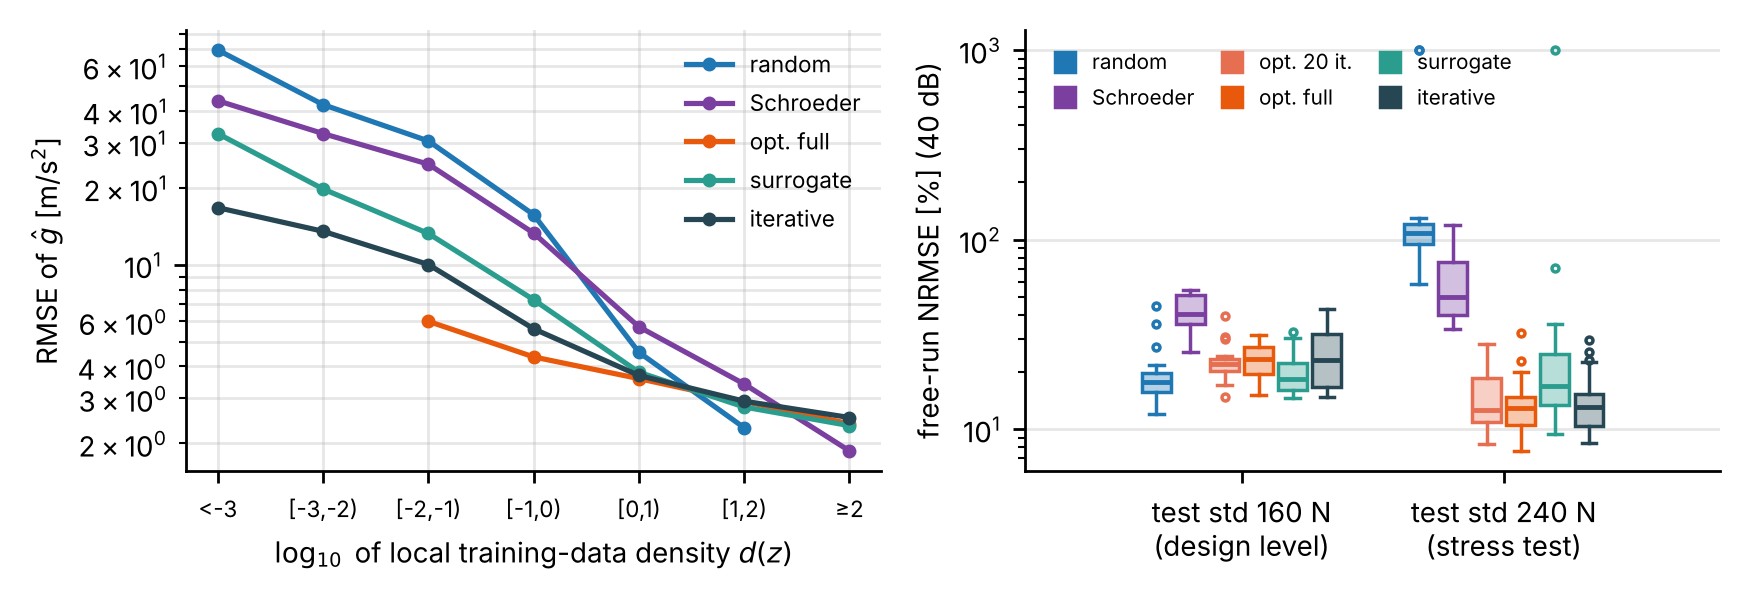
\includegraphics[width=0.85\textwidth]{fig_ext_mechanism.png}\\[2pt]
\small (b)
\caption{Extension, \mNExt{} seeds. (a) Left: one-step error of the identified force law over $\Dz$ for each
design and noise level. Right: model error vs.\ the space-filling cost achieved on the true system (40\,dB,
all designs and seeds). (b) Left: RMSE of $\hat g$ against the local density $d(z)$ of the training data
(40\,dB, pooled over seeds). Right: free-run simulation error on unseen random-phase multisines at the design
level (160\,N) and at 1.5$\times$ (240\,N); diverged runs are plotted at $10^3$\,\%.}
\label{fig:ext}\end{figure*}

\textbf{E1: coverage becomes accuracy.} Table~\ref{tab:ext} and Fig.~\ref{fig:ext}a: at 40\,dB the
median one-step error over $\Dz$ falls from \mXRfortyeuni\,\% (random) and \mXSfortyeuni\,\% (Schroeder)
to \mXOfullfortyeuni\,\% (optimised), a median paired improvement of \mFOfullforty$\times$
(\mWinOfullfortyeuni/\mNExt{} seeds better, $p$\,\mPOfullfortyeuni). The early-stopped designs, which
match the paper's cost level, already give \mFOtwentyforty$\times$, so most of the gain comes from the
first iterations. Schroeder also beats random phases over $\Dz$ (\mFSforty$\times$), but far less. The gain shrinks with noise (\mFOfullinf$\times$ clean, \mFOfullthirty$\times$ at
30\,dB) but stays significant. It is not an artefact of the cross-validated ridge parameter: with the same
fixed $\lambda$ for every design the gain is \mFixFAforty$\times$ ($\lambda=10^{-6}$) and
\mFixFBforty$\times$ ($\lambda=10^{-4}$) at 40\,dB. The Schroeder result, however, is sensitive to $\lambda$
(\mFixSAforty\,\% vs.\ \mFixSBforty\,\%), and its error even drops at 30\,dB, where cross-validation picks a
larger $\lambda$: for designs that leave parts of $\Dz$ empty, $e_{\mathrm{uni}}$ measures extrapolation, and
that depends on the regulariser. Fig.~\ref{fig:ext}b (left) shows the mechanism: for every design the error
falls with the local data density; the random-phase input leaves large parts of $\Dz$ at densities below
$10^{-2}$, where the model only extrapolates, while the optimised input leaves almost none.

\textbf{The price.} On free-run tests at the design level the picture changes: the random-phase test
signals live exactly where random-phase training data are dense, and there the random-phase model is as
good as or better than the optimised one (\mXRfortyesimonesixty\,\% vs.\
\mXOfullfortyesimonesixty\,\%; not significant at 1\,\%, $p$\mPwOfullfortyesimonesixty). The space-filling input spends the same number of samples on a larger
region, which is a bias--variance trade-off, not a free gain. At 1.5$\times$ the amplitude the
random-phase model fails (median \mXRfortyesimtwoforty\,\%, \mXRfortydivTot{} of its 200 free-run
simulations diverged) while the optimised one stays at \mXOfullfortyesimtwoforty\,\% with no divergence.
Schroeder, with the lowest crest factor, gives the worst free-run model at the design level
(\mXSfortyesimonesixty\,\%): it covers $x_1,x_2$ but not the input axis.

\textbf{E2: the design still works when the model is unknown.} Designing on a model identified from one
random-phase period keeps a \mFOsurforty$\times$ improvement (\mXOsurfortyeuni\,\%), even though the
surrogate predicts the coverage poorly: the true cost of \st{Osur} is \mXOsurfortyCtrue{} while the
surrogate predicted \mChatOsur; \mXOsurfortydivTot{} of its 200 free-run simulations diverged. One
re-identification round (\st{Oiter}) moves the true cost to \mXOiterfortyCtrue{} and the gain to
\mFOiterforty$\times$. Running 100 iterations on the first surrogate (\st{Osur100}) gives
\mFOsurOneZeroZeroforty$\times$ (true cost \mXOsurOneZeroZerofortyCtrue): the optimiser lowers the
\emph{surrogate's} cost, partly by exploiting its errors outside the data. The budgets differ: \st{Osur} and
\st{Osur100} use two experiments, \st{Oiter} three and 40 surrogate iterations; every final model is still
identified from one period of the last experiment only. In our runs, a second identification round gained
more than 80 extra iterations on the first surrogate; we did not test this difference statistically.

\textbf{E3: the cost predicts model quality, but only coarsely.} Across design families the space-filling
cost on the true system ranks the model error (pooled Spearman $\rho=\mRhoforty$ at 40\,dB, \mRhoinf{} clean,
\mRhothirty{} at 30\,dB; Fig.~\ref{fig:ext}a right; descriptive only, as the seeds of one design are not
independent families). It also holds within the random-phase designs ($\rho=\mRhoInR$) and over the
three optimised stopping points together ($\rho=\mRhoOpt$, $p$\mRhoOptP), but among the converged designs
alone it disappears ($\rho=\mRhoInOfull$, $p$\mRhoInPOfull): once $\Dz$ is well covered, further cost
reductions no longer predict the error. The cost is therefore a useful indicator of whether a dataset covers
$\Dz$, not a fine predictor of model accuracy; it also needs the measured or simulated states, so it can
only be checked after the experiment or on a model.


\FloatBarrier
\section{Discussion and Limitations}
\textbf{What was learned.} The method of \citet{Kiss2024} is reproducible from the paper alone: every
qualitative finding and every number that does not depend on the stopping point agrees. The one
quantitative gap is in how far the optimisation is run, which the paper does not report. A reproduction
should therefore report the optimiser budget and the stopping rule as carefully as the model.

\textbf{Threats to validity.} (i) The authors' optimiser options, $\epsilon$, steady-state rule and
seeds are unknown; we fixed our choices in the M2 protocol before seeing results and tested the most
influential ones ($\epsilon$, optimiser, budget, grid, initial state). (ii) H1 is supported by two
independent budget-limited optimisers, but \texttt{fmincon}'s interior-point steps were not reproduced
exactly; without MATLAB it remains a hypothesis. (iii) The Fig.~8 values of the paper were read from the
axes. (iv) The extension uses one system, one model class and simulated white sensor noise. Noisy states
in the regressors could bias least squares (errors-in-variables, \citealp{Soderstrom2007}); E4 shows that this
bias is small here and that the noise error is mostly variance, amplified by $\sqrt2/T_s$ in the target. With
a fixed absolute noise level, designs that spread the states more also have a higher effective SNR; the
noise-free case (\mFOfullinf$\times$) isolates the coverage effect. (v) The surrogate design used short runs (20 iterations); longer runs on a fixed
surrogate helped little, and a second identification round appeared more useful (unequal budgets, not tested statistically). (vi) The converged
optima depend on the machine (\S3), so only statistics over seeds, not single converged values, should be
compared.

\textbf{Unsuccessful attempts} (kept in the package): $P=5$ violated the steady-state rule for the
optimised signal; a first gradient check with a too small step reported false errors; PyTorch could
not be installed, so all gradients were derived by hand. An early test of the extension pipeline on seed 0 used
state-relative SNR, which penalises designs that excite the system more. After seeing that test we changed to
fixed absolute sensor noise, because a real sensor's noise does not depend on the input; this was a choice
made after an early result, and the noise-free case, which does not depend on it, shows the same ranking.

\textbf{Research use.} The extension suggests a practical recipe for robotics and UAV identification,
where the dynamics are unknown and test time is expensive: one short random-phase experiment, a local
model, then one or two space-filling redesigns on the identified model.


\section{Conclusion}
\textbf{Answer to the reproduction question: largely yes.} Secs.~4.4--4.6 of \citet{Kiss2024} are reproduced by an independent Python
implementation: coverage plots, initial costs, Schroeder crest factor and Monte-Carlo trend agree
(T1, T3--T5 reproduced; T6 Schroeder crest factor reproduced, optimised crest factor partially). The converged optimised cost is lower than published (\mCfullMed{} vs.\ 3.88);
budget-limited optimisers stop in the paper's cost range, so T2 and T7 are partially reproduced; early
stopping by the authors (H1) is consistent with this but cannot be proven without their settings. The stated 69$\times$ should read 74$\times$.

\textbf{Extension.} Better coverage does give better models: with the same input spectrum, the model
identified from the space-filling input is \mFOfullforty$\times$ more accurate over the region of
interest (40\,dB, \mFOfullinf$\times$ noise-free) and much more robust to larger inputs, at a moderate
cost (about one third higher free-run error) on test signals of the random-phase kind. The benefit survives when the true system is unknown and the design is computed on an
identified model (\mFOsurforty$\times$, \mFOiterforty$\times$ with one re-identification round), and the
space-filling cost ranks design families by model error ($\rho=\mRhoforty$) but does not resolve
differences among already well-covering designs. The gain survives an actuator peak limit at the Schroeder
crest factor (\mPkOneNineF$\times$), and the remaining noise error is variance that periodic averaging removes,
not a bias that needs instrumental variables.


{\footnotesize
\bibliographystyle{plainnat}
\setlength{\bibsep}{1pt}
\bibliography{refs}}

{\footnotesize\textbf{Reproducibility.} Code, data-generation scripts, seeds, versions and every figure/number
in this report: \texttt{M4\_g202622300\_Reproducibility\_Package.zip} (\texttt{README.md}; one main script
\texttt{python code/run\_all.py}). Software: Python 3.13, NumPy \citep{Harris2020}, SciPy \citep{Virtanen2020},
Numba \citep{Lam2015}, Matplotlib \citep{Hunter2007}, PyVista \citep{Sullivan2019} (Fig.~\ref{fig:sys}a only).
No data, code or figures of the authors are used or redistributed; all data are simulated.

\textbf{Authorship and AI-use statement.} This is my individual work. I selected the paper, set the
protocol (M2) and every setting, ran all experiments, checked every result against the paper and can explain
all code and results. Claude (Anthropic) was used, as allowed by the course rules, to draft and debug the
Python code from my protocol, to propose the extension design that I then fixed, to draft and format this
report and the figures, and, as a separate Claude instance that had not written the work, to review it
(recomputing numbers from the result files and checking the literature). I verified the derivations (adjoint
gradient, ridge LS), the unit tests (gradient checks against finite differences), the related-work citations,
and every number, which is generated automatically from the result files.\par}
\end{document}
